%% if you are submitting an initial manuscript then you should have submission as an option here
%% if you are submitting a revised manuscript then you should have revision as an option here
%% otherwise options taken by the article class will be accepted
\documentclass[submission]{FPSAC2020}
%% but DO NOT pass any options (or change anything else anywhere) which alters page size / layout / font size etc

%% note that the class file already loads {amsmath, amsthm, amssymb}

\newtheorem{theorem}{Theorem}
\newtheorem{lemma}[theorem]{Lemma}
\newtheorem{proposition}[theorem]{Proposition}
\newtheorem{definition}[theorem]{Definition}
\newtheorem{example}[theorem]{Example}
\newtheorem{corollary}[theorem]{Corollary}
\newtheorem{conjecture}[theorem]{Conjecture}
\newtheorem{remark}[theorem]{Remark}

\usepackage{paralist} % special lists
\usepackage{xargs} % commands with optional parameters
\usepackage{ulem}\normalem % special underline
\usepackage{picins/picins}
\graphicspath{{figures/}{figures/diagonals/}{figures/walks/}{figures/tubes/}}
\usepackage{nicefrac}
\usepackage[export]{adjustbox}
\usepackage{tikz}
\usetikzlibrary{matrix}
\makeatletter
\protected\def\tikz@nonactivesemicolon{\ifmmode\mathrel{\mathop\ordinarysemicolon}\else;\fi} 
\makeatother
\usepackage{overpic}
\usepackage{wasysym, pifont}

% math special letters
\newcommand{\R}{\mathbb{R}} % reals
\newcommand{\Q}{\mathbb{Q}} % rationals
\newcommand{\N}{\mathbb{N}} % naturals
\newcommand{\Z}{\mathbb{Z}} % integers
\newcommand{\C}{\mathbb{C}} % complex
\newcommand{\f}[1]{{\mathfrak{#1}}} % mathfrak letters
%\newcommand{\cal}[1]{{\mathcal{#1}}} % call letters
\renewcommand{\b}[1]{{\boldsymbol{#1}}} % bold letters

% math commands
\newcommand{\set}[2]{\left\{ #1 \;\middle|\; #2 \right\}} % set notation
\newcommand{\bigset}[2]{\big\{ #1 \;|\; #2 \big\}} % big set notation
\newcommand{\biggset}[2]{\bigg\{ #1 \;\bigg|\; #2 \bigg\}} % bigg set notation
\newcommand{\Bigset}[2]{\Big\{ #1 \;\Big|\; #2 \Big\}} % Big set notation
\newcommand{\ssm}{\smallsetminus} % small set minus
\newcommand{\dotprod}[2]{\langle \, #1 \; | \; #2 \, \rangle} % dot product
\newcommand{\symdif}{\,\triangle\,} % symmetric difference
\newcommand{\one}{{1\!\!1}} % the all one vector
\newcommand{\eqdef}{\mbox{\,\raisebox{0.2ex}{\scriptsize\ensuremath{\mathrm:}}\ensuremath{=}\,}} % :=
\newcommand{\defeq}{\mbox{~\ensuremath{=}\raisebox{0.2ex}{\scriptsize\ensuremath{\mathrm:}} }} % =:
\newcommand{\interior}[1]{\mathring{#1}} % interior

% others
\newcommand{\ie}{\textit{i.e.}~} % id est
\newcommand{\eg}{\textit{e.g.}~} % exempli gratia
\newcommand{\Eg}{\textit{E.g.}~} % Exempli gratia
\newcommand{\aka}{\textit{a.k.a.}~} % also known as
\newcommand{\viceversa}{\textit{vice versa}} % exempli gratia
\newcommand{\red}{\color{red}} % red command
\newcommand{\blue}{\color{blue}} % blue command
\newcommand{\green}{\color{green}} % green command
\newcommand{\defn}[1]{\uline{\textit{#1}}} % emphasis of a definition
\newcommand{\parabf}[1]{\noindent\textbf{#1}.} % paragraph bf

% type cones
\newcommandx{\Fan}[1][1=F]{\mathcal{#1}} % fan
\newcommandx{\ray}[1][1=r]{\b{#1}} % ray
\newcommandx{\rays}[1][1=R]{\b{#1}} % rays
\newcommand{\gvector}[1]{\b{g}(#1)} % g-vector of #1
\newcommand{\gvectorFull}[2]{\b{g}(#1,#2)} % g-vector of #2 wrt #1
\newcommand{\gvectors}[1]{\b{g}(#1)} % g-vectors of #1
\newcommand{\gvectorsFull}[2]{\b{g}(#1,#2)} % g-vectors of #2 wrt #1
\newcommandx{\gvectorFan}[1][1=\quiver]{\mathcal{F}(#1)} % g-vector fan
\newcommand{\typeCone}{\mathbb{TC}} % type cone
\newcommandx{\coefficient}[3][1={\ray[s]}, 2=\ray, 3=\ray']{\alpha_{#2,#3}(#1)} 
\newcommandx{\Asso}[2][1=n,2={}]{\mathsf{Asso}^{#2}(#1)} % associahedron
\newcommandx{\clusterAlgebra}[1][1=\B_\circ]{\mathcal{A}\!\left(#1\right)} % cluster algebra
\newcommand{\seed}{\Sigma} % a cluster
\newcommand{\cluster}{X} % a cluster
\newcommandx{\clusters}{X} % all clusters
\newcommand{\B}{B} % b-matrix
\newcommandx{\meshes}[1][1=\B_\circ]{\mathcal{M}(#1)} % meshes
\newcommandx{\variables}[1][1=\B_\circ]{\mathcal{V}(#1)} % all variables
\newcommand{\coefficients}{\mathrm{P}} % a coefficients tuple
\newcommand*\circled[1]{\tikz[baseline=(char.base)]{\node[shape=circle, draw, inner sep=1.5pt, scale=.7] (char) {#1};}}
\newcommand{\compactVectorD}[2]{\begin{bmatrix} #1 \\ #2 \end{bmatrix}}
\newcommand{\compactVectorT}[3]{\begin{bmatrix} #1 \\[-.1cm] #2 \\[-.1cm] #3 \end{bmatrix}}
\newcommand{\quiver}{\bar Q} % quiver
\newcommand{\blossom}{^\text{\ding{96}}} % blossom
\newcommandx{\walks}[1][1=\quiver]{\mathcal{W}(#1)} % walks
\newcommandx{\strings}[1][1=\quiver]{\mathcal{S}(#1)} % strings
\newcommand{\hL}{\text{\rotatebox[origin=c]{180}{\checked}}}
\newcommand{\hR}{\text{\rotatebox[origin=c]{180}{\reflectbox{\checked}}}}
\newcommand{\cL}{\text{\reflectbox{\checked}}}
\newcommand{\cR}{\text{\checked}}
\newcommand{\hh}[1]{\hL#1\hR} % hook - hook
\newcommand{\cc}[1]{\cL#1\cR} % cohook - cohook
\newcommand{\hc}[1]{\hL#1\cR} % hook - cohook
\newcommand{\ch}[1]{\cL#1\hR} % cohook - hook
\renewcommand{\top}{\mathrm{top}} % top
\newcommand{\bottom}{\mathrm{bot}} % bottom
\newcommandx{\NKC}[1][1=\quiver]{\mathcal{NK}(#1)} % non-kissing complex
\newcommand{\peaks}[1]{\mathsf{peaks}(#1)} % peaks
\newcommand{\deeps}[1]{\mathsf{deeps}(#1)} % deeps
\newcommand{\multiplicityVector}{\b{m}} % multiplicity vector
\newcommand{\ground}{V} % ground set
\newcommandx{\graphG}[1][1=G]{#1} % graph
\newcommandx{\tube}[1][1=t]{#1} % tube
\newcommandx{\tubes}[1][1=\graphG]{\mathcal{T}(#1)} % all tubes
\newcommandx{\tubing}[1][1=T]{#1} % tubing
\newcommand{\connectedComponents}{\kappa} % connected components
\newcommand{\nestedComplex}{\mathcal{N}} % nested complex
\newcommand{\nonDisconnecting}{\mathrm{nd}} % non-disconnecting vertices

%% define your title in the usual way
\title{On type cones of $\b{g}$-vector fans}

%% define your authors in the usual way
%% use \addressmark{1}, \addressmark{2} etc for the institutions, and use \thanks{} for contact details
\author[Arnau Padrol, Yann Palu, Vincent Pilaud and Pierre-Guy Plamondon]{
	Arnau Padrol\thanks{\href{mailto:arnau.padrol@imj-prg.fr}{arnau.padrol@imj-prg.fr}. Supp. by ANR grant CAPPS~(17\,CE40\,0018).}\addressmark{1},
	\stepcounter{footnote}%
	Yann Palu\thanks{\href{mailto:yann.palu@u-picardie.fr}{yann.palu@u-picardie.fr}. Supp. by ANR grant SC3A~(15\,CE40\,0004\,01).}\addressmark{2}, \\
	Vincent Pilaud\thanks{\href{mailto:vincent.pilaud@lix.polytechnique.fr}{vincent.pilaud@lix.polytechnique.fr}. Supp. by ANR SC3A~15\,CE40\,0004\,01 and CAPPS~17\,CE40\,0018.}\addressmark{3}
	\and
	Pierre-Guy Plamondon\thanks{\href{mailto:pierre-guy.plamondon@math.u-psud.fr}{pierre-guy.plamondon@math.u-psud.fr}. Supp. by ANR grant SC3A~(15\,CE40\,0004\,01).}\addressmark{4},
}


%% then use \addressmark to match authors to institutions here
\address{
	\addressmark{1} Institut de Math�matiques de Jussieu - Paris Rive Gauche, Sorbonne Universit\'e, Paris, France \\
	\addressmark{2} LAMFA, Universit\'e Picardie Jules Verne, Amiens, France \\
	\addressmark{3} CNRS \& LIX, \'Ecole Polytechnique, Palaiseau, France \\
	\addressmark{4} Laboratoire de Math\'ematiques d'Orsay, CNRS, Universit\'e Paris-Saclay, France
}

%% put the date of submission here
\received{\today}

%% leave this blank until submitting a revised version
%\revised{}

%% put your English abstract here, or comment this out if you don't have one yet
%% please don't use custom commands in your abstract / resume, as these will be displayed online
%% likewise for citations -- please don't use \cite, and instead write out your citation as something like (author year)
\abstract{
We study the type cone (\ie the space of all polytopal realizations) of $\b{g}$-vector fans of finite type cluster-like complexes (finite type cluster complexes, non-kissing complexes of gentle algebra, and graphical nested complexes). We show that this cone is often simplicial, which explains an elegant ``kinematic'' construction of the associahedron as a section of a high dimensional positive orthant by certain affine subspaces parametrized by a low dimensional positive orthant.
}

%% put your French abstract here, or comment this out if you don't have one
\resumetitle{R\'esum\'e}
\resume{
Nous \'etudions le type cone (\ie l'espace de toutes les r\'ealisations polytopales) des \'eventails de $\b{g}$-vecteurs de complexes de type amass�s (complexes amass�s de type fini, complexes platoniques d'alg\`ebres aimables, et complexes emboit\'es graphi\-ques). Nous montrons que ce cone est souvent simplicial, ce qui explique une \'el\'egante construction ``cin\'ematique'' de l'associa\`edre comme section d'un orthant positif de haute dimension par certains sous-espaces affines param\`etr�s par un orthant positif de basse dimension.
}

%% put your keywords here, or comment this out if you don't have them yet
\keywords{Fans $\cdot$ cluster algebras $\cdot$ non-kissing complexes $\cdot$ graph associahedra}

%% you can include your bibliography however you want, but using an external .bib file is STRONGLY RECOMMENDED and will make the editor's life much easier
%% regardless of how you do it, please use numerical citations, ie. [xx, yy] in the text

%% this sample uses biblatex, which (among other things) takes care of URLs in a more flexible way than bibtex
%% but you can use bibtex if you want
\usepackage[backend=bibtex, firstinits=true, maxbibnames=99]{biblatex}
\DeclareFieldFormat[article,inbook,incollection,inproceedings,patent,thesis,unpublished]{title}{\textit{#1}\isdot}
\renewbibmacro{in:}{}
\addbibresource{typeConeAssociahedraFPSAC.bib}
%% note the \printbibliography command at the end of the file which goes with these biblatex commands

\begin{document}

\maketitle
%% note that you DO NOT have to put your abstract here -- it is generated by \maketitle and the \abstract and \resume commands above

\section{Introduction}

This paper focuses on a surprising construction of the associahedron that recently appeared in mathematical physics.
Motivated by the prediction of the behavior of scattering particles, N.~Arkani-Hamed, Y.~Bai, S.~He, and G.~Yan recently described in~\cite[Sect.~3.2]{ArkaniHamedBaiHeYan} the kinematic associahedron.
It is a class of polytopal realizations of the classical associahedron obtained as sections of a high-dimensional positive orthant with well-chosen affine subspaces.
This construction provides a large degree of freedom in the choice of the parameters defining these affine subspaces, and actually produces all polytopes whose normal fan is affinely equivalent to that of J.-L.~Loday's associahedron~\cite{Loday} (see \cref{subsec:associahedra}).
These realizations were then extended by V.~Bazier-Matte, G.~Douville, K.~Mousavand, H.~Thomas and E.~Y\i ld\i r\i m~\cite{BazierMatteDouvilleMousavandThomasYildirim} in the context of finite type cluster algebras (see \cref{subsec:generalizedAssociahedra}) using tools from quiver representation theory.

We revisit, extend and explore further this construction using a reversed approach.
Given a complete simplicial fan~$\Fan$, we consider the space~$\typeCone(\Fan)$ of all its polytopal realizations.
This space was called type cone in~\cite{McMullen-typeCone} and deformation cone in~\cite{Postnikov}, who studied the case when~$\Fan$ is the braid arrangement leading to the rich theory of generalized permutahedra.
The type cone is known to be a polyhedral cone defined by a collection of inequalities corresponding to the linear dependences among the rays of~$\Fan$ contained in pairs of adjacent maximal cones of~$\Fan$ (see \cref{def:typeCone}).
Our approach is based on an elementary but powerful observation: for any fan~$\Fan$, all polytopal realizations of~$\Fan$ can be described as sections of a high dimensional positive orthant with a collection of affine subspaces parametrized by the type cone~$\typeCone(\Fan)$ (see \cref{prop:alternativePolytopalRealization}); if moreover the type cone~$\typeCone(\Fan)$ is a simplicial cone, it leads to a simple parametrization of all polytopal realizations of~$\Fan$ by a positive orthant corresponding to the facets of the type cone~$\typeCone(\Fan)$ (see \cref{coro:simplicialTypeCone}).
To prove that the type cone~$\typeCone(\Fan)$ is simplicial, we just need to identify which pairs of adjacent maximal cones of~$\Fan$ correspond to the facets of~$\typeCone(\Fan)$ and to show that the corresponding linear dependences among their rays positively span the linear dependence among the rays of any pair of adjacent maximal cones of~$\Fan$.
When applied to cluster algebras (see \cref{subsec:generalizedAssociahedra}), this yields all polytopal realizations of the $\b{g}$-vector fans, revisiting and extending results of~\cite{BazierMatteDouvilleMousavandThomasYildirim}.

This new perspective has several advantages, as our proof uniformly applies to \emph{any initial seed} (acyclic or not), \emph{any finite type cluster algebra} (simply-laced or not), and \emph{any positive real-valued parameters} (rational or not). In contrast, note that the result of~\cite{BazierMatteDouvilleMousavandThomasYildirim} is first proved for acyclic initial seeds in simply-laced cluster algebras for integer parameters, and then extended by a technical folding argument to all finite types and by an approximation argument to arbitrary real-valued parameters.
These advantages of the type cone approach all follow from one essential feature: it enables to completely separate the algebraic aspects from the geometric aspects of the problem.

Besides revisiting the construction of~\cite{ArkaniHamedBaiHeYan, BazierMatteDouvilleMousavandThomasYildirim} and extending it to any initial seed, our type cone approach is also successful when applied to the $\b{g}$-vector fans of other families of generalizations of the associahedron.
In the present paper, we explore specifically the non-kissing complexes of gentle algebras introduced in~\cite{PaluPilaudPlamondon-nonkissing} (see \cref{subsec:gentleAssociahedra}) and the graphical nested complexes studied in~\cite{CarrDevadoss, FeichtnerSturmfels, Postnikov, Zelevinsky} (see \cref{subsec:graphAssociahedra}).

Many details and all proofs are omitted in this extended abstract for space reason, but a complete treatment can be found in~\cite{PadrolPaluPilaudPlamondon}.
In particular, the quiver representation theory is an iceberg in this abstract: while useful for intuition and essential for certain proofs (\eg \cref{thm:meshMutations}), it is mostly hidden and only appears in the Auslander-Reiten quivers used to represent the inequalities of the type cones (in \cref{fig:labelFacetDefiningInequalititiesAsso,fig:labelFacetDefiningInequalititiesCA,fig:labelFacetDefiningInequalititiesNKC}).

\section{Type cone of a fan}
\label{sec:typeCone}

Fix an essential complete simplicial fan\footnote{A \defn{polyhedral cone} is the positive span of finitely many vectors or equivalently, the intersection of finitely many closed linear half-spaces. The \defn{faces} of a cone are its intersections with its supporting hyperplanes. A \defn{fan}~$\Fan$ is a set of polyhedral cones such that any face of a cone of~$\Fan$ belongs to~$\Fan$, and any two cones of~$\Fan$ intersect along a face of both. A fan is \defn{essential} if the intersection of its cones is the origin, \defn{complete} if the union of its cones covers~$\R^n$, and \defn{simplicial} if all its cones are generated by dimension many rays.}~$\Fan$ in~$\R^n$. Let~$\b{G}$ be the $N \times n$-matrix whose rows are (representative vectors of) the rays of~$\Fan$.
% and let~$\b{K}$ be a $(N-n) \times N$-matrix that spans the left kernel of~$\b{G}$ (\ie $\b{K}\b{G} = 0$). 
For any height vector~$\b{h} \in \R^N$, we define the polytope\footnote{A \defn{polytope} is the convex hull of finitely many points or equivalently, a bounded intersection of finitely many closed affine half-spaces.}
\(
P_\b{h} \eqdef \set{\b{x} \in \R^n}{\b{G}\b{x} \le \b{h}}.
\)
Unfortunately, the normal fan\footnote{The \defn{normal cone} of a face~$F$ of a polytope~$P$ is the cone generated by the normal vectors of the facets of~$P$ containing~$F$. The \defn{normal fan} of~$P$ is the set of normal cones of all its faces.} of this polytope~$P_\b{h}$ does not always coincide with the fan~$\Fan$ we started from. The following statement gives a simple characterization of the height vectors~$h$ for which it is the case. It is a reformulation of regularity of triangulations of vector configurations, introduced in the theory of secondary polytopes~\cite{GelfandKapranovZelevinsky}.
We present here a convenient formulation from~\cite{ChapotonFominZelevinsky}.

\begin{proposition}
\label{prop:characterizationPolytopalFan}
Let~$\Fan$ be an essential complete simplicial fan in~$\R^n$. Then the following are equivalent for any height vector~$\b{h} \in \R^N$:
\begin{compactenum}
\item The fan~$\Fan$ is the normal fan of the polytope~$P_\b{h} \eqdef \set{\b{x} \in \R^n}{\b{G}\b{x} \le \b{h}}$.
\item For any two adjacent maximal cones~$\R_{\ge0}\rays$ and~$\R_{\ge0}\rays'$ of~$\Fan$ with~$\rays \ssm \{\ray\} = \rays' \ssm \{\ray'\}$, we have
\(
{\displaystyle\sum}_{\ray[s] \in \rays \cup \rays'} \coefficient[{\ray[s]}][\rays][\rays'] \, h_{\ray[s]} > 0,
\)
where
\(
{\displaystyle\sum}_{\ray[s] \in \rays \cup \rays'} \coefficient[{\ray[s]}][\rays][\rays'] \, \ray[s] = 0
\)
is the unique linear dependence among the rays of~$\rays \cup \rays'$ such that~$\coefficient[{\ray[r]}][\rays][\rays'] + \coefficient[{\ray[r]'}][\rays][\rays'] = 2$. 
\end{compactenum}
\end{proposition}

\begin{definition}[\cite{McMullen-typeCone}]
\label{def:typeCone}
The \defn{type cone} of~$\Fan$ is the cone~$\typeCone(\Fan)$ of all polytopal realizations of~$\Fan$:
\begin{align*}
\typeCone(\Fan) & \eqdef \set{\b{h} \in \R^N}{\Fan \text{ is the normal fan of } P_\b{h}} \\
& = \Bigset{\b{h} \in \R^N}{\sum_{\ray[s] \in \rays \cup \rays'} \coefficient[{\ray[s]}][\rays][\rays'] \, \b{h}_{\ray[s]} > 0 \; \begin{array}{l} \text{for any adjacent maximal} \\ \text{cones~$\R_{\ge0}\rays$ and~$\R_{\ge0}\rays'$ of~$\Fan$} \end{array}}.
\end{align*}
\end{definition}

Note that the type cone is an open cone and contains a lineality subspace of dimension~$n$ (it is invariant by translation in~$\b{G} \R^n$). Therefore, we say that the type cone is \defn{simplicial} when it has precisely $N-n$ facets.

\begin{definition}
An \defn{extremal adjacent pair} of~$\Fan$ is a pair of adjacent maximal cones~$\R_{\ge0}\rays, \R_{\ge0}\rays'$ of~$\Fan$ such that the corresponding inequality ${\displaystyle\sum}_{\ray[s] \in \rays \cup \rays'} \coefficient[{\ray[s]}][\rays][\rays'] \, \b{h}_{\ray[s]} > 0$ in the definition of the type cone~$\typeCone(\Fan)$ actually defines a facet of~$\typeCone(\Fan)$.
In other words, extremal adjacent pairs define the extremal rays of the polar of the closed type cone~$\typeCone(\Fan)$.
\vspace{.2cm}
\end{definition}

\begin{example}
\label{exm:typeCone}
Consider the $2$-dimensional fan~$\Fan$ depicted in \cref{fig:typeCone} (left).
% (we will encounter this fan again in \cref{exm:typeConeCoarsenings,exm:typeConeMinkowskiSum,exm:typeConeAsso}).
It has five rays labeled~$1, \dots, 5$ and five maximal cones labeled~$a,\dots, e$.
Its type cone~$\typeCone(\Fan)$ lies in~$\R^5$, but has a $2$-dimensional lineality space, and is defined by the following five inequalities:
\begin{gather*}
H^>_{ab}: \; \b{h}_1 + \b{h}_3 - \b{h}_2 > 0
\qquad
H^>_{bc}: \; \b{h}_2 + \b{h}_4 - \b{h}_3 > 0
\qquad
H^>_{cd}: \; \b{h}_3 + \b{h}_5 - \b{h}_4 > 0
\\
H^>_{de}: \; \b{h}_1 + \b{h}_4 > 0
\qquad
H^>_{ae}: \; \b{h}_2 + \b{h}_5 > 0,
\end{gather*}
where $H^>_{xy}$ denotes the halfspace defined by the inequality corresponding to the two adjacent maximal cones~$x$ and~$y$.
%Note that the inequalities~$H^>_{ae}$ and~$H^>_{de}$ are redundant, while the other three define facets, so that the extremal adjacent pairs are~$(a,b)$, $(b,c)$ and~$(c,d)$.
For example, the height vector~$(\nicefrac{1}{2}, \nicefrac{3}{4}, \nicefrac{5}{4}, 1, \nicefrac{5}{4})$ belongs to~$\typeCone(\Fan)$, and the corresponding polytope is represented in \cref{fig:typeCone} (middle).
To represent $\typeCone(\Fan)$, we slice it with a transversal $2$-dimensional affine space, and obtain the red triangle in \cref{fig:typeCone} (right).

\begin{figure}[t]
	\centerline{{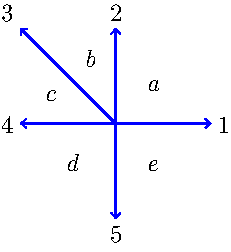
\includegraphics[scale=1]{typeConeFan}} \quad {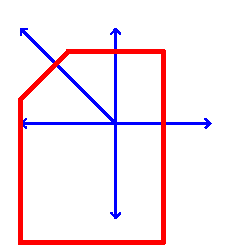
\includegraphics[scale=1]{typeConePolytope}} \quad \raisebox{.5cm}{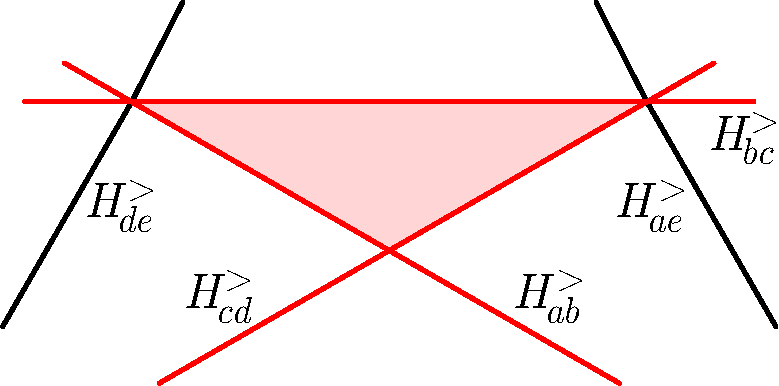
\includegraphics[scale=.45]{typeCone}}}
	\caption{A $2$-dimensional fan~$\Fan$ with five rays $1, \dots, 5$ and five maximal cones~$a, \dots, e$ (left), its polytopal realization corresponding to the height vector~$(\nicefrac{1}{2}, \nicefrac{3}{4}, 1, 1, \nicefrac{5}{4})$ (middle), and a $2$-dimensional slice of the type cone~$\typeCone(\Fan)$ (right).}
	\label{fig:typeCone}
\end{figure}
\end{example}

\begin{remark}
All fans considered in \cref{sec:gvectorFans} have the \defn{unique exchange relation property}: the linear dependence ${\displaystyle\sum}_{\ray[s] \in \rays \cup \rays'} \coefficient[{\ray[s]}][\rays][\rays'] \, \ray[s] = 0$ only depends on the exchanged rays~$\ray[r]$ and~$\ray[r]'$, not on the maximal adjacent cones~$\rays$ and~$\rays'$. We then write~$\coefficient[{\ray[s]}][\ray][\ray']$ instead of~$\coefficient[{\ray[s]}][\rays][\rays']$ and we call \defn{extremal exchangeable pairs} of~$\Fan$ the pairs of exchangeable rays~$\ray, \ray'$ of~$\Fan$ such that the corresponding inequality ${\displaystyle\sum}_{\ray[s] \in \rays \cup \rays'} \coefficient[{\ray[s]}][\ray][\ray'] \, \b{h}_{\ray[s]} > 0$ defines a facet of~$\typeCone(\Fan)$.

\end{remark}

To conclude this section, we consider alternative polytopal realizations of the fan~$\Fan$ and discuss their behavior in the situation when the type cone~$\typeCone(\Fan)$ is simplicial.
Fix a $(N-n) \times N$-matrix~$\b{K}$ that spans the left kernel of the $N \times n$-matrix~$\b{G}$ (\ie $\b{K}\b{G} = 0$). 

\begin{proposition}
\label{prop:alternativePolytopalRealization}
The map~$\b{x} \in \R^n \mapsto \b{h} - G\b{x} \in \R^N$ is an affine transformation of the polytope~$P_\b{h} \eqdef \set{\b{x} \in \R^n}{\b{G}\b{x} \le \b{h}}$ to the polytope~$Q_\b{h} \eqdef \set{\b{z} \in \R^N}{\b{K}\b{z} = \b{K}\b{h} \text{ and } \b{z} \ge 0}$.
\end{proposition}

\begin{corollary}
\label{coro:simplicialTypeCone}
Assume that the type cone~$\typeCone(\Fan)$ is simplicial and consider inner normal vectors to its $N-n$ facets. Since all these vectors belong to the left kernel of~$\b{G}$ by \cref{prop:characterizationPolytopalFan}, we can assume that they are the rows of the ${(N-n) \times N}$-matrix~$\b{K}$. Then, for any positive vector~${\b{\ell} \in \R_{>0}^{N-n}}$, the polytope
\(
R_\b{\ell} \eqdef \set{\b{z} \in \R^N}{K\b{z} = \b{\ell} \text{ and } \b{z} \ge 0}
\)
is a realization of the fan~$\Fan$.
Moreover, the polytopes~$R_\b{\ell}$ for~$\b{\ell} \in \R_{>0}^{N-n}$ describe all polytopal realizations of~$\Fan$.
\end{corollary}

\section{Applications to $\b{g}$-vector fans}
\label{sec:gvectorFans}

We now study the type cones of the normal fans of three families generalizing the associahedron constructed in~\cite{Loday}: the generalized associahedra of finite type cluster algebras~\cite{FominZelevinsky-ClusterAlgebrasI, FominZelevinsky-ClusterAlgebrasII, FominZelevinsky-ClusterAlgebrasIV, HohlwegLangeThomas, HohlwegPilaudStella}, the gentle associahedra~\cite{PaluPilaudPlamondon-nonkissing}, and the graph associahedra~\mbox{\cite{CarrDevadoss, FeichtnerSturmfels, Postnikov, Zelevinsky}}.
%All these families contain the classical associahedra~$\Asso[n]$ constructed in~\cite{Loday}.

\subsection{Classical associahedra}
\label{subsec:associahedra}

%We start with the classical associahedron.
An $n$-dimensional \defn{associahedron} is a polytope whose face lattice is the reverse inclusion lattice of dissections (\ie sets of pairwise non-crossing diagonals) of a convex~$(n+3)$-gon.
In particular, its vertices correspond to triangulations of the $(n+3)$-gon and its facets correspond to internal diagonals of the $(n+3)$-gon.
Let~$X(n) \eqdef \set{(a,b)}{0 \le a < b \le n+2}$ denote all diagonals of the $(n+3)$-gon and~$Y(n) \eqdef \set{(a,b)}{0 \le a < b-2 \le n} \subset X(n)$.
The \defn{$\b{g}$-vector} of a diagonal $(a,b) \in X(n)$ is ${\gvector{a,b} \eqdef {\displaystyle\sum}_{\,a < \ell < b} \b{e}_\ell - \frac{b-a-1}{n+1} {\displaystyle\sum}_{\,1 \le \ell \le n+1} \b{e}_\ell}$.
%Note that~$\gvector{a,b} = 0$ if~$(a,b)$ is not internal.
We set~$\gvector{D} \eqdef \set{\gvector{a,b}}{(a,b) \in D}$ for a dissection~$D$.
Recall that:
\begin{compactitem}
\item the set of cones
\(
\gvectorFan[n] \eqdef \bigset{\R_{\ge0} \, \gvectors{D}}{D \text{ dissection of the $(n+3)$-gon}}
\)
forms a complete simplicial fan.
See \cref{fig:lodayFans}\,(left and middle).

\item the fan~$\gvectorFan[n]$ is the normal fan of the associahedron~$\Asso[n]$ constructed \eg in~\cite{Loday}.

\item for any two adjacent triangulations~$T$ and~$T'$ with~${T \ssm \{(a,b)\} = T' \ssm \{(a',b')\}}$ such that~${0 \le a < a' < b < b' \le n+2}$, the linear dependence among the $\b{g}$-vectors of~${T \cup T'}$ is given by
\(
\gvector{a,b} + \gvector{a',b'} = \gvector{a,b'} + \gvector{a',b}.
\)
\end{compactitem}

\smallskip
This provides a redundant description of the type cone of the fan~$\gvectorFan[n]$.

%For~$n \in \N$, we define~$X(n) \eqdef \set{(a,b)}{0 \le a < b \le n+2}$ and $Y(n) \eqdef \set{(a,b)}{0 \le a < b-2 \le n}$.

\begin{corollary}
\label{coro:typeConeAsso}
%Let~$n \in \N$ and~$X(n) \eqdef \set{(a,b)}{0 \le a < b \le n+2}$. 
For any~$n \in \N$, the type cone of the fan~$\gvectorFan[n]$ is given by
\[
\typeCone \big( \gvectorFan[n] \big) = \set{\b{h} \in \R^{X(n)} \!}{\begin{array}{@{}l@{}} \b{h}_{(0,n+2)} = 0, \qquad\text{and}\qquad \b{h}_{(a,a+1)} = 0 \text{ for all } 0 \le a \le n+1 \\ \b{h}_{(a,b)} \! + \! \b{h}_{(a',b')} \! > \! \b{h}_{(a,b')} \! + \! \b{h}_{(a',b)} \text{ for all } 0 \! \le \! a \! < \! a' \! < \! b \! < \! b' \! \le \! n+2 \end{array}} \!.
\]
\end{corollary}

The next statement, illustrated in \cref{fig:labelFacetDefiningInequalititiesAsso}, gives the facets of the type cone of~$\gvectorFan[n]$.

%\begin{example}
%\label{exm:typeConeAsso}
%The type cone of~$\gvectorFan[2]$ (resp.~$\gvectorFan[3]$) lives in~$\R^5$ (resp.~$\R^9$), has a lineality space of dimension~$2$ (resp.~$3$), and has $3$ (resp.~$6$) facet-defining inequalities described in \cref{prop:extremalExchangeablePairsAsso}.
%We represent these inequalities in red in \cref{fig:labelFacetDefiningInequalititiesAsso}, using incoming and outgoing arrows to distinguish their left and right hand sides.
%For instance, the inequality~$\red \circled{A}$ is given by~$\b{h}_{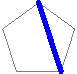
\includegraphics[scale=.3]{diagonalA1}} + \b{h}_{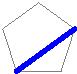
\includegraphics[scale=.3]{diagonalA3}} > \b{h}_{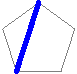
\includegraphics[scale=.3]{diagonalA2}}$.

%\centerline{
%	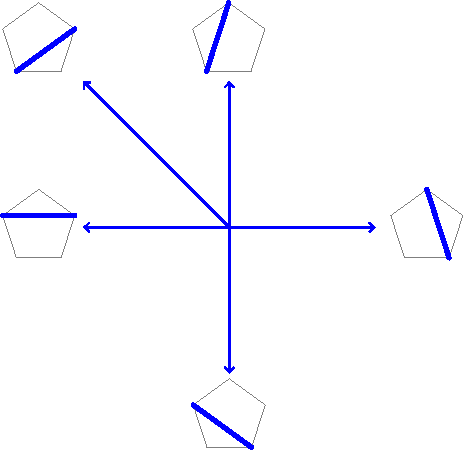
\includegraphics[scale=.5]{lodayFan2}
%%	\quad
%%	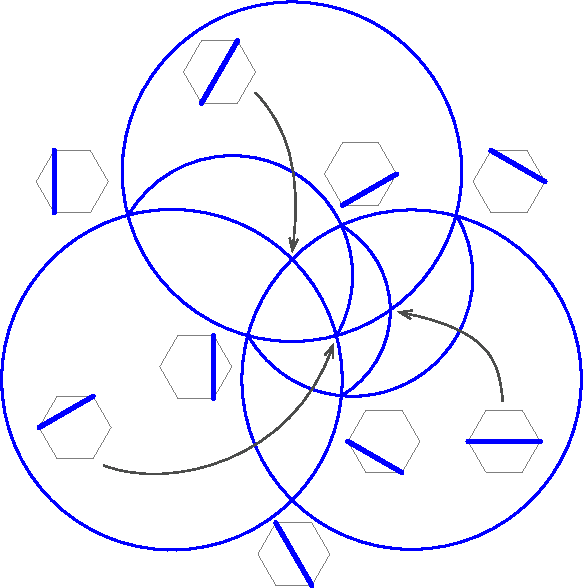
\includegraphics[scale=.5]{lodayFan3}
%	\quad
%	\begin{tikzpicture}
%		\matrix (m) [matrix of math nodes, row sep=.35cm, column sep=.2cm, nodes={anchor=center, align=center, inner sep=0pt}, ampersand replacement=\&]{
%			\& \;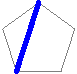
\includegraphics[scale=.7]{diagonalA2} \& \node (b) {\red \circled{B}}; \& \;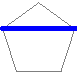
\includegraphics[scale=.7]{diagonalA4} \& \\
%			\;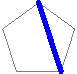
\includegraphics[scale=.7]{diagonalA1} \& \node (a) {\red \circled{A}}; \& \;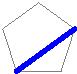
\includegraphics[scale=.7]{diagonalA3} \& \node (c) {\red \circled{C}}; \& \;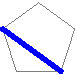
\includegraphics[scale=.7]{diagonalA5} \\};
%		\draw[->] (m-2-1) -- (m-1-2);
%		\draw[->] (m-1-2) -- (m-2-3);
%		\draw[->] (m-2-3) -- (m-1-4);
%		\draw[->] (m-1-4) -- (m-2-5);
%		\draw[red] (a) -- (m-2-1);
%		\draw[red] (a) -- (m-2-3);
%		\draw[red] (a) -- (m-1-2);
%		\draw[red] (b) -- (m-1-2);
%		\draw[red] (b) -- (m-1-4);
%		\draw[red] (b) -- (m-2-3);
%		\draw[red] (c) -- (m-2-3);
%		\draw[red] (c) -- (m-2-5);
%		\draw[red] (c) -- (m-1-4);
%	\end{tikzpicture}
%}
%
%%\begin{center}
%%	\raisebox{-2.9cm}{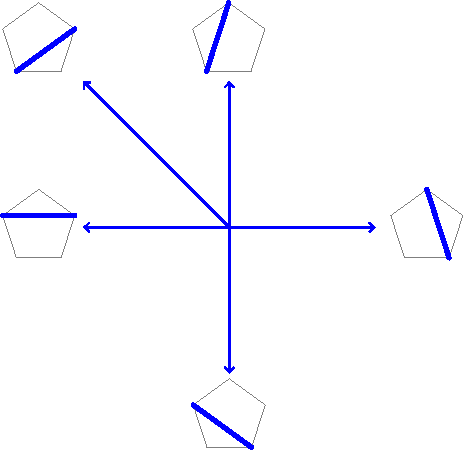
\includegraphics[scale=.8]{lodayFan2}}
%%	\begin{minipage}{10cm}
%%	\(
%%	\begin{array}{r|cccccc}
%%	\text{diagonals} & \raisebox{-.25cm}{\;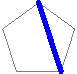
\includegraphics[scale=.7]{diagonalA1}}  & \raisebox{-.25cm}{\;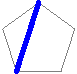
\includegraphics[scale=.7]{diagonalA2}} & \raisebox{-.25cm}{\;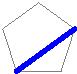
\includegraphics[scale=.7]{diagonalA3}} & \raisebox{-.25cm}{\;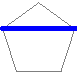
\includegraphics[scale=.7]{diagonalA4}} & \raisebox{-.25cm}{\;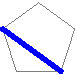
\includegraphics[scale=.7]{diagonalA5}} \\[.3cm]
%%	\text{$\b{g}$-vectors} & \compactVectorD{1}{0} & \compactVectorD{0}{1} & \compactVectorD{-1}{1} & \compactVectorD{-1}{0} & \compactVectorD{0}{-1} \\[.6cm]
%%	\text{facet}		& 1 & -1 & 1 & 0 & 0 & \red \circled{A} \\
%%	\text{defining} 	& 0 & 1 & -1 & 1 & 0 & \red \circled{B} \\
%%	\text{inequalities}	& 0 & 0 & 1 & -1 & 1 & \red \circled{C} \\[.2cm]
%%	\end{array}
%%	\)
%%	\\
%%	\hspace*{2.3cm}
%%	\begin{tikzpicture}
%%		\matrix (m) [matrix of math nodes, row sep=.35cm, column sep=.2cm, nodes={anchor=center, align=center, inner sep=0pt}]{
%%			& \;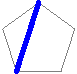
\includegraphics[scale=.7]{diagonalA2} & \node (b) {\red \circled{B}}; & \;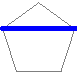
\includegraphics[scale=.7]{diagonalA4} & \\
%%			\;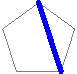
\includegraphics[scale=.7]{diagonalA1} & \node (a) {\red \circled{A}}; & \;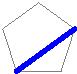
\includegraphics[scale=.7]{diagonalA3} & \node (c) {\red \circled{C}}; & \;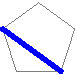
\includegraphics[scale=.7]{diagonalA5} \\};
%%		\draw[->] (m-2-1) -- (m-1-2);
%%		\draw[->] (m-1-2) -- (m-2-3);
%%		\draw[->] (m-2-3) -- (m-1-4);
%%		\draw[->] (m-1-4) -- (m-2-5);
%%		\draw[red] (a) -- (m-2-1);
%%		\draw[red] (a) -- (m-2-3);
%%		\draw[red] (a) -- (m-1-2);
%%		\draw[red] (b) -- (m-1-2);
%%		\draw[red] (b) -- (m-1-4);
%%		\draw[red] (b) -- (m-2-3);
%%		\draw[red] (c) -- (m-2-3);
%%		\draw[red] (c) -- (m-2-5);
%%		\draw[red] (c) -- (m-1-4);
%%	\end{tikzpicture}
%%	\end{minipage}
%%\end{center}
%\end{example}


\begin{proposition}
\label{prop:extremalExchangeablePairsAsso}
Two internal diagonals~$(a,b)$ and~$(a',b')$ of the~$(n+3)$-gon form an extremal exchangeable pair for the fan~$\gvectorFan[n]$ if and only if~$a = a'+1$ and~$b = b'+1$, or the opposite.
\end{proposition}

\begin{corollary}
\label{coro:simplicialTypeConeAsso}
The type cone~$\typeCone \big( \gvectorFan[n] \big)$ is simplicial.
\end{corollary}

Combining \cref{coro:simplicialTypeCone,coro:simplicialTypeConeAsso} and \cref{prop:extremalExchangeablePairsAsso}, we derive the following description of all polytopal realizations of~$\gvectorFan[n]$, recovering all associahedra of~\cite[Sect.~3.2]{ArkaniHamedBaiHeYan}.
%Note that the arguments of~\cite[Sect.~3.2]{ArkaniHamedBaiHeYan} were quite different from the present~approach.

\begin{corollary}[{\cite[Sect.~3.2]{ArkaniHamedBaiHeYan}}]
\label{coro:allPolytopalRealizationsAsso}
%Let~$X(n) \eqdef \set{(a,b)}{0 \le a < b \le n+2}$ and $Y(n) \eqdef \set{(a,b)}{0 \le a < b-2 \le n}$.
For any~$n \in \N$ and any~$\b{\ell} \in \R_{>0}^{Y(n)}$, the polytope
\[
R_\b{\ell}(n) \eqdef \set{\b{z} \in \R^{X(n)} \!}{\begin{array}{@{}l@{}} \b{z} \ge 0, \quad \b{z}_{(0,n+2)} = 0 \quad\text{and}\quad \b{z}_{(a,a+1)} = 0 \text{ for all } 0 \le a \le n+1 \\ \b{z}_{(a,b-1)} + \b{z}_{(a+1,b)} - \b{z}_{(a,b)} - \b{z}_{(a+1,b-1)} = \b{\ell}_{(a,b)} \text{ for all } (a,b) \in Y(n) \end{array}}
\]
is an $n$-dimensional associahedron, whose normal fan is~$\gvectorFan[n]$.
Moreover, the polytopes~$R_\b{\ell}(n)$ for~$\b{\ell} \in \R_{>0}^{Y(n)}$ describe all polytopal realizations of the fan~$\gvectorFan[n]$.
\end{corollary}

\begin{figure}[t]
	\centerline{
	\raisebox{.5cm}{\begin{overpic}[scale=.5]{lodayFan2} \put(0,105){$\boxed{n=2}$} \end{overpic}}
	\hspace{.5cm}
	\begin{overpic}[scale=.5]{lodayFan3} \put(-10,93){$\boxed{n=3}$} \end{overpic}
	\hspace{.5cm}
	\raisebox{.35cm}{\begin{overpic}[scale=.5]{clusterFanA}
		\put(75,92){$\boxed{\B_\circ \! = \!\! {\tiny\left[\begin{array}{@{}r@{}r@{}r@{}} 0 & -1 & 1 \\ 1 & 0 & -1 \\ -1 & 1 & 0 \end{array}\right]}}$}
		\put(35,33){${\scriptstyle x_1}$}
		\put(47,54){${\scriptstyle x_2}$}
		\put(59,33){${\scriptstyle x_3}$}
		\put(70,37){$\frac{x_2 + x_3}{x_1}$}
		\put(22,18){$\frac{x_1 + x_3}{x_2}$}
		\put(29,62){$\frac{x_1 + x_2}{x_3}$}
		\put(80,57){$\frac{x_1 + x_2 + x_3}{x_1 x_3}$}
		\put(35,-7){$\frac{x_1 + x_2 + x_3}{x_1 x_2}$}
		\put(-10,57){$\frac{x_1 + x_2 + x_3}{x_2 x_3}$}
%		\put(34,49){$x_1$}
%		\put(57,61){$x_2$}
%		\put(57,36){$x_3$}
%		\put(68,33){$\frac{x_2 + x_3}{x_1}$}
%		\put(17,36){$\frac{x_1 + x_3}{x_2}$}
%		\put(44,74){$\frac{x_1 + x_2}{x_3}$}
%		\put(90,49){$\frac{x_1 + x_2 + x_3}{x_1 x_3}$}
%		\put(7,12){$\frac{x_1 + x_2 + x_3}{x_1 x_2}$}
%		\put(7,84){$\frac{x_1 + x_2 + x_3}{x_2 x_3}$}
	\end{overpic}}
	}
	\caption{The fans~$\gvectorFan[2]$, $\gvectorFan[3]$ and~$\gvectorFan[\B_\circ]$. The two right $3$-dimensional fans are intersected with the sphere and stereographically projected from the direction~$(-1,-1,-1)$.}
	\label{fig:lodayFans}
	\vspace*{-.2cm}
\end{figure}

\begin{figure}
	\centerline{
%	\begin{minipage}[b]{9cm}
%	\begin{center}
%	${\red \circled{B}}: \; \b{h}_{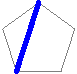
\includegraphics[scale=.3]{diagonalA2}} + \b{h}_{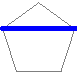
\includegraphics[scale=.3]{diagonalA4}} > \b{h}_{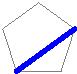
\includegraphics[scale=.3]{diagonalA3}}$	
%	\\[.1cm]
%	${\red \circled{A}}: \; \b{h}_{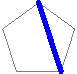
\includegraphics[scale=.3]{diagonalA1}} + \b{h}_{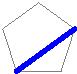
\includegraphics[scale=.3]{diagonalA3}} > \b{h}_{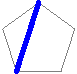
\includegraphics[scale=.3]{diagonalA2}}$
%	\qquad
%	${\red \circled{C}}: \; \b{h}_{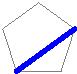
\includegraphics[scale=.3]{diagonalA3}} + \b{h}_{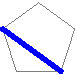
\includegraphics[scale=.3]{diagonalA5}} > \b{h}_{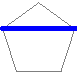
\includegraphics[scale=.3]{diagonalA4}}$
%	\\
	\begin{tikzpicture}
		\matrix (m) [matrix of math nodes, row sep=.35cm, column sep=.2cm, nodes={anchor=center, align=center, inner sep=0pt}, ampersand replacement=\&]{
			$\!\!\boxed{n=2}\!\!$ \\
			\& \;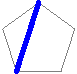
\includegraphics[scale=.7]{diagonalA2} \& \node (b) {\red \circled{B}}; \& \;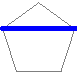
\includegraphics[scale=.7]{diagonalA4} \& \\
			\;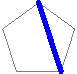
\includegraphics[scale=.7]{diagonalA1} \& \node (a) {\red \circled{A}}; \& \;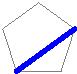
\includegraphics[scale=.7]{diagonalA3} \& \node (c) {\red \circled{C}}; \& \;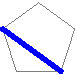
\includegraphics[scale=.7]{diagonalA5} \\};
		\draw[->] (m-3-1) -- (m-2-2);
		\draw[->] (m-2-2) -- (m-3-3);
		\draw[->] (m-3-3) -- (m-2-4);
		\draw[->] (m-2-4) -- (m-3-5);
		\draw[red, -<] (a) -- (m-3-1);
		\draw[red, -<] (a) -- (m-3-3);
		\draw[red, ->] (a) -- (m-2-2);
		\draw[red, -<] (b) -- (m-2-2);
		\draw[red, -<] (b) -- (m-2-4);
		\draw[red, ->] (b) -- (m-3-3);
		\draw[red, -<] (c) -- (m-3-3);
		\draw[red, -<] (c) -- (m-3-5);
		\draw[red, ->] (c) -- (m-2-4);
	\end{tikzpicture}
%	\end{center}
%	\end{minipage}
%	\hspace{-.5cm}
	\quad
	\begin{tikzpicture}
		\matrix (m) [matrix of math nodes, row sep=.35cm, column sep=.2cm, nodes={anchor=center, align=center, inner sep=0pt}, ampersand replacement=\&]{
			$\!\!\boxed{n=3}\!\!$ \&\& \;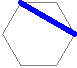
\includegraphics[scale=.7]{diagonalB3} \& \node (c) {\red \circled{C}}; \& \;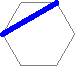
\includegraphics[scale=.7]{diagonalB7} \&\& \\
			\& \;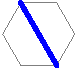
\includegraphics[scale=.7]{diagonalB2} \& \node (b) {\red \circled{B}}; \& \;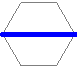
\includegraphics[scale=.7]{diagonalB5} \& \node (e) {\red \circled{E}}; \& \;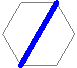
\includegraphics[scale=.7]{diagonalB8} \& \\
			\;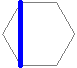
\includegraphics[scale=.7]{diagonalB1} \& \node (a) {\red \circled{A}}; \& \;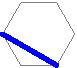
\includegraphics[scale=.7]{diagonalB4} \& \node (d) {\red \circled{D}}; \& \;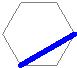
\includegraphics[scale=.7]{diagonalB6} \& \node (f) {\red \circled{F}}; \& \;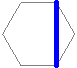
\includegraphics[scale=.7]{diagonalB9} \\};
		\draw[->] (m-3-1) -- (m-2-2);
		\draw[->] (m-2-2) -- (m-1-3);
		\draw[->] (m-2-2) -- (m-3-3);
		\draw[->] (m-1-3) -- (m-2-4);
		\draw[->] (m-3-3) -- (m-2-4);
		\draw[->] (m-2-4) -- (m-1-5);
		\draw[->] (m-2-4) -- (m-3-5);
		\draw[->] (m-1-5) -- (m-2-6);
		\draw[->] (m-3-5) -- (m-2-6);
		\draw[->] (m-2-6) -- (m-3-7);
		\draw[red, -<] (a) -- (m-3-1);
		\draw[red, -<] (a) -- (m-3-3);
		\draw[red, ->] (a) -- (m-2-2);
		\draw[red, -<] (b) -- (m-2-2);
		\draw[red, -<] (b) -- (m-2-4);
		\draw[red, ->] (b) -- (m-1-3);
		\draw[red, ->] (b) -- (m-3-3);
		\draw[red, -<] (c) -- (m-1-3);
		\draw[red, -<] (c) -- (m-1-5);
		\draw[red, ->] (c) -- (m-2-4);
		\draw[red, -<] (d) -- (m-3-3);
		\draw[red, -<] (d) -- (m-3-5);
		\draw[red, ->] (d) -- (m-2-4);
		\draw[red, -<] (e) -- (m-2-4);
		\draw[red, -<] (e) -- (m-2-6);
		\draw[red, ->] (e) -- (m-1-5);
		\draw[red, ->] (e) -- (m-3-5);
		\draw[red, -<] (f) -- (m-3-5);
		\draw[red, -<] (f) -- (m-3-7);
		\draw[red, ->] (f) -- (m-2-6);
	\end{tikzpicture}
	}
	\caption{Facet-defining inequalities of the type cone~$\typeCone \big( \gvectorFan[n] \big)$. See \cref{prop:extremalExchangeablePairsAsso}. Each circled red letter gives an inequality with left (resp.~right) hand side given by the incoming (resp.~outgoing) arrows. For instance, the inequality~$\red \textcircled{\scriptsize A}$ is~$\b{h}_{\protect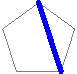
\includegraphics[scale=.3]{diagonalA1}} + \b{h}_{\protect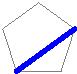
\includegraphics[scale=.3]{diagonalA3}} > \b{h}_{\protect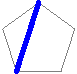
\includegraphics[scale=.3]{diagonalA2}}$.}
	\label{fig:labelFacetDefiningInequalititiesAsso}
	\vspace*{-.4cm}
\end{figure}

\subsection{Cluster fan and generalized associahedra}
\label{subsec:generalizedAssociahedra}

We now consider finite type cluster algebras, defined by S.~Fomin and A.~Zelevinsky in~\cite{FominZelevinsky-ClusterAlgebrasI, FominZelevinsky-ClusterAlgebrasII}.
We skip the technical definitions and refer to the original papers for details.
We fix an initial exchange matrix~$\B_\circ$ (acyclic or not) of finite type and denote by~$\clusterAlgebra$ the corresponding cluster algebra with principal coefficients, and by~$\variables$ its cluster variables. We denote by~$\gvectorFull{\B_\circ}{x}$ the \defn{$\b{g}$-vector} of a cluster variable~$x \in \variables$ as defined in~\cite{FominZelevinsky-ClusterAlgebrasIV}, and we set~$\gvectorFull{\B_\circ}{\cluster} \eqdef \set{\gvectorFull{\B_\circ}{x}}{x \in \cluster}$ for a cluster~$\cluster$ of~$\clusterAlgebra$. Recall~that:
\begin{compactenum}
\item the set of cones
\(
\bigset{\R_{\ge0} \, \gvectorsFull{\B_\circ}{\cluster}}{\cluster \text{ cluster of } \clusterAlgebra \!},
\)
together with all their faces, forms a complete simplicial fan~$\gvectorFan[\B_\circ]$, called the \defn{cluster fan} of~$\B_\circ$.
See \cref{fig:lodayFans}.

\item the cluster fan~$\gvectorFan[\B_\circ]$ is the normal fan of the \defn{generalized associahedron}~$\Asso[\B_\circ]$, constructed for bipartite (resp.~acyclic, resp.~arbitrary) initial exchange matrices in~\cite{ChapotonFominZelevinsky} (resp.~\cite{HohlwegLangeThomas}, resp.~\cite{HohlwegPilaudStella}).

\item for any two adjacent seeds~${(\B, \cluster)}$ and~${(\B', \cluster')}$ in $\clusterAlgebra$ with~$\cluster \ssm \{x\} = \cluster' \ssm \{x'\}$, the $\b{g}$-vectors of~$\cluster \cup \cluster'$ with respect to~$\B_\circ$ satisfy one of the two linear dependences
\[
\smash{\gvectorFull{\B_\circ}{x} + \gvectorFull{\B_\circ}{x'} = \!\!\!\! \sum_{\substack{y \in \cluster \cap \cluster' \\ b_{xy} < 0}} \!\!\! -b_{xy} \, \gvectorFull{\B_\circ}{y}
\quad\text{or}\quad
\gvectorFull{\B_\circ}{x} + \gvectorFull{\B_\circ}{x'} = \!\!\!\! \sum_{\substack{y \in \cluster \cap \cluster' \\ b_{xy} > 0}} \!\!\! b_{xy} \, \gvectorFull{\B_\circ}{y}.}
\]
\end{compactenum}

This provides a redundant description of the type cone of the cluster fan~$\gvectorFan[\B_\circ]$.
Denoting by~$\b{n}(\B_\circ, x, x')$ the vector whose coefficients are given by the appropriate linear dependence above, we obtain the following statement.

\begin{corollary}
\label{coro:typeConeCA}
For any finite type exchange matrix~$\B_\circ$, the type cone of~$\gvectorFan[\B_\circ]$ is given by
\[
\typeCone \big( \gvectorFan[\B_\circ] \big) = \bigset{\b{h} \in \R^{\variables}}{\dotprod{\b{n}(\B_\circ, x, x')}{\b{h}} > 0 \text{ for any exchangeable variables } x, x'}.
\]
\end{corollary}

%%\parpic(7cm,6cm)(10pt, 140pt)[r][b]{
%%	\begin{overpic}[scale=.5]{clusterFanA}
%%		\put(34,49){$x_1$}
%%		\put(57,61){$x_2$}
%%		\put(57,36){$x_3$}
%%		\put(68,33){$\frac{x_2 + x_3}{x_1}$}
%%		\put(17,36){$\frac{x_1 + x_3}{x_2}$}
%%		\put(44,74){$\frac{x_1 + x_2}{x_3}$}
%%		\put(90,49){$\frac{x_1 + x_2 + x_3}{x_1 x_3}$}
%%		\put(7,12){$\frac{x_1 + x_2 + x_3}{x_1 x_2}$}
%%		\put(7,84){$\frac{x_1 + x_2 + x_3}{x_2 x_3}$}
%%	\end{overpic}
%%}{
%\begin{example}
%Consider the cluster fan~$\gvectorFan[\B_\circ]$ for the initial exchange matrix of type~$A_3$ cyclic represented on the right.
%%As it is a $3$-dimensional fan, we intersect it with the unit sphere and project the result stereographically from the pole $(-1,-1,-1)$.
%Its type cone lives in~$\R^{9}$ and has a lineality space of dimension~$3$.
%It has $6$ facet-defining inequalities (given below), which correspond to the mesh mutations of \cref{thm:extremalExchangeablePairsCA}.
%
%\begin{figure}[h]
%	\newcommand{\fitClusterVariable}[1]{\parbox[c][.7cm][c]{1.5cm}{\centering $#1$}}
%	\centerline{
%    \begin{tikzpicture}
%    	\matrix (m) [matrix of math nodes, row sep=.4cm, column sep=-.1cm, nodes={anchor=center, align=center, inner sep=0pt}, ampersand replacement=\&]{
%    		\fitClusterVariable{\phantom{1}} \& \node (e1) {\red \circled{E}}; \& \fitClusterVariable{\frac{x_1 + x_2 + x_3}{x_2 x_3}} \&\& \fitClusterVariable{x_3} \& \node (c) {\red \circled{C}}; \& \fitClusterVariable{\frac{x_1 + x_2 + x_3}{x_1 x_3}} \&\& \fitClusterVariable{x_1} \& \node (a2) {\red \circled{A}}; \& \fitClusterVariable{\phantom{1}} \\
%    		\& \fitClusterVariable{\frac{x_1 + x_2}{x_3}} \& \node (f1) {\red \circled{F}}; \& \fitClusterVariable{\frac{x_1 + x_3}{x_2}} \& \node (b) {\red \circled{B}}; \& \fitClusterVariable{\frac{x_2 + x_3}{x_1}} \& \node (d) {\red \circled{D}}; \& \fitClusterVariable{\frac{x_1 + x_2}{x_3}} \& \node (f2) {\red \circled{F}}; \& \fitClusterVariable{\frac{x_1 + x_3}{x_2}} \\
%    		\fitClusterVariable{\phantom{1}} \&\& \fitClusterVariable{x_1} \& \node (a1) {\red \circled{A}}; \& \fitClusterVariable{\frac{x_1 + x_2 + x_3}{x_1 x_2}} \&\& \fitClusterVariable{x_2} \& \node (e2) {\red \circled{E}}; \& \fitClusterVariable{\frac{x_1 + x_2 + x_3}{x_2 x_3}} \&\& \fitClusterVariable{\phantom{1}} \\};
%    	\draw[densely dotted, thick] (m-1-1) -- (m-2-2);
%    	\draw[densely dotted, thick] (m-3-1) -- (m-2-2);
%    	\draw[->] (m-2-2) -- (m-1-3);
%    	\draw[->] (m-2-2) -- (m-3-3);
%    	\draw[->] (m-1-3) -- (m-2-4);
%    	\draw[->] (m-3-3) -- (m-2-4);
%    	\draw[->] (m-2-4) -- (m-1-5);
%    	\draw[->] (m-2-4) -- (m-3-5);
%    	\draw[->] (m-1-5) -- (m-2-6);
%    	\draw[->] (m-3-5) -- (m-2-6);
%    	\draw[->] (m-2-6) -- (m-1-7);
%    	\draw[->] (m-2-6) -- (m-3-7);
%    	\draw[->] (m-1-7) -- (m-2-8);
%    	\draw[->] (m-3-7) -- (m-2-8);
%    	\draw[->] (m-2-8) -- (m-1-9);
%    	\draw[->] (m-2-8) -- (m-3-9);
%    	\draw[->] (m-1-9) -- (m-2-10);
%    	\draw[->] (m-3-9) -- (m-2-10);
%    	\draw[densely dotted, thick] (m-2-10) -- (m-1-11);
%    	\draw[densely dotted, thick] (m-2-10) -- (m-3-11);
%    	\draw[red] (a1) -- (m-3-3);
%    	\draw[red] (a1) -- (m-3-5);
%    	\draw[red] (a1) -- (m-2-4);
%    	\draw[red] (a2) -- (m-1-9);
%    	\draw[red, densely dotted, thick] (a2) -- (m-1-11);
%    	\draw[red] (a2) -- (m-2-10);
%    	\draw[red] (b) -- (m-2-4);
%    	\draw[red] (b) -- (m-2-6);
%    	\draw[red] (b) -- (m-1-5);
%    	\draw[red] (b) -- (m-3-5);
%    	\draw[red] (c) -- (m-1-5);
%    	\draw[red] (c) -- (m-1-7);
%    	\draw[red] (c) -- (m-2-6);
%    	\draw[red] (d) -- (m-2-6);
%    	\draw[red] (d) -- (m-2-8);
%    	\draw[red] (d) -- (m-1-7);
%    	\draw[red] (d) -- (m-3-7);
%    	\draw[red, densely dotted, thick] (e1) -- (m-1-1);
%    	\draw[red] (e1) -- (m-1-3);
%    	\draw[red] (e1) -- (m-2-2);
%    	\draw[red] (e2) -- (m-3-7);
%    	\draw[red] (e2) -- (m-3-9);
%    	\draw[red] (e2) -- (m-2-8);
%    	\draw[red] (f1) -- (m-2-2);
%    	\draw[red] (f1) -- (m-2-4);
%    	\draw[red] (f1) -- (m-1-3);
%    	\draw[red] (f1) -- (m-3-3);
%    	\draw[red] (f2) -- (m-2-8);
%    	\draw[red] (f2) -- (m-2-10);
%    	\draw[red] (f2) -- (m-1-9);
%    	\draw[red] (f2) -- (m-3-9);
%    \end{tikzpicture}
%    }
%	\caption{Facet-defining inequalities of the type cone~$\typeCone \big( \gvectorFan[n] \big)$. See \cref{prop:extremalExchangeablePairsAsso}. See \cref{fig:labelFacetDefiningInequalititiesAsso} for the conventions.}
%	\label{fig:labelFacetDefiningInequalititiesAsso}
%\end{figure}
%
%\end{example}
%%}

To describe the facets of this type cone, we need the following special mutations.

\begin{figure}[b]
	\newcommand{\fitClusterVariable}[1]{\parbox[c][.7cm][c]{1.6cm}{\centering $#1$}}
	\centerline{
    \begin{tikzpicture}
    	\matrix (m) [matrix of math nodes, row sep=.4cm, column sep=-.1cm, nodes={anchor=center, align=center, inner sep=0pt}, ampersand replacement=\&]{
    		\fitClusterVariable{\phantom{1}} \& \node (e1) {\red \circled{E}}; \& \fitClusterVariable{\frac{x_1 + x_2 + x_3}{x_2 x_3}} \&\& \fitClusterVariable{x_3} \& \node (c) {\red \circled{C}}; \& \fitClusterVariable{\frac{x_1 + x_2 + x_3}{x_1 x_3}} \&\& \fitClusterVariable{x_1} \& \node (a2) {\red \circled{A}}; \& \fitClusterVariable{\phantom{1}} \\
    		\& \fitClusterVariable{\frac{x_1 + x_2}{x_3}} \& \node (f1) {\red \circled{F}}; \& \fitClusterVariable{\frac{x_1 + x_3}{x_2}} \& \node (b) {\red \circled{B}}; \& \fitClusterVariable{\frac{x_2 + x_3}{x_1}} \& \node (d) {\red \circled{D}}; \& \fitClusterVariable{\frac{x_1 + x_2}{x_3}} \& \node (f2) {\red \circled{F}}; \& \fitClusterVariable{\frac{x_1 + x_3}{x_2}} \\
    		\fitClusterVariable{\phantom{1}} \&\& \fitClusterVariable{x_1} \& \node (a1) {\red \circled{A}}; \& \fitClusterVariable{\frac{x_1 + x_2 + x_3}{x_1 x_2}} \&\& \fitClusterVariable{x_2} \& \node (e2) {\red \circled{E}}; \& \fitClusterVariable{\frac{x_1 + x_2 + x_3}{x_2 x_3}} \&\& \fitClusterVariable{\phantom{1}} \\};
    	\draw[densely dotted, thick] (m-1-1) -- (m-2-2);
    	\draw[densely dotted, thick] (m-3-1) -- (m-2-2);
    	\draw[->] (m-2-2) -- (m-1-3);
    	\draw[->] (m-2-2) -- (m-3-3);
    	\draw[->] (m-1-3) -- (m-2-4);
    	\draw[->] (m-3-3) -- (m-2-4);
    	\draw[->] (m-2-4) -- (m-1-5);
    	\draw[->] (m-2-4) -- (m-3-5);
    	\draw[->] (m-1-5) -- (m-2-6);
    	\draw[->] (m-3-5) -- (m-2-6);
    	\draw[->] (m-2-6) -- (m-1-7);
    	\draw[->] (m-2-6) -- (m-3-7);
    	\draw[->] (m-1-7) -- (m-2-8);
    	\draw[->] (m-3-7) -- (m-2-8);
    	\draw[->] (m-2-8) -- (m-1-9);
    	\draw[->] (m-2-8) -- (m-3-9);
    	\draw[->] (m-1-9) -- (m-2-10);
    	\draw[->] (m-3-9) -- (m-2-10);
    	\draw[densely dotted, thick] (m-2-10) -- (m-1-11);
    	\draw[densely dotted, thick] (m-2-10) -- (m-3-11);
    	\draw[red, -<] (a1) -- (m-3-3);
    	\draw[red, -<] (a1) -- (m-3-5);
    	\draw[red, ->] (a1) -- (m-2-4);
    	\draw[red, -<] (a2) -- (m-1-9);
    	\draw[red, densely dotted, thick] (a2) -- (m-1-11);
    	\draw[red, ->] (a2) -- (m-2-10);
    	\draw[red, -<] (b) -- (m-2-4);
    	\draw[red, -<] (b) -- (m-2-6);
    	\draw[red, ->] (b) -- (m-1-5);
    	\draw[red, ->] (b) -- (m-3-5);
    	\draw[red, -<] (c) -- (m-1-5);
    	\draw[red, -<] (c) -- (m-1-7);
    	\draw[red, ->] (c) -- (m-2-6);
    	\draw[red, -<] (d) -- (m-2-6);
    	\draw[red, -<] (d) -- (m-2-8);
    	\draw[red, ->] (d) -- (m-1-7);
    	\draw[red, ->] (d) -- (m-3-7);
    	\draw[red, densely dotted, thick] (e1) -- (m-1-1);
    	\draw[red, -<] (e1) -- (m-1-3);
    	\draw[red, ->] (e1) -- (m-2-2);
    	\draw[red, -<] (e2) -- (m-3-7);
    	\draw[red, -<] (e2) -- (m-3-9);
    	\draw[red, ->] (e2) -- (m-2-8);
    	\draw[red, -<] (f1) -- (m-2-2);
    	\draw[red, -<] (f1) -- (m-2-4);
    	\draw[red, ->] (f1) -- (m-1-3);
    	\draw[red, ->] (f1) -- (m-3-3);
    	\draw[red, -<] (f2) -- (m-2-8);
    	\draw[red, -<] (f2) -- (m-2-10);
    	\draw[red, ->] (f2) -- (m-1-9);
    	\draw[red, ->] (f2) -- (m-3-9);
    \end{tikzpicture}
    }
    % \vspace{-.1cm}
	\caption{The facet-defining inequalities of the type cone~$\typeCone \big( \gvectorFan[\B_\circ] \big)$ for the cluster fan of \cref{fig:lodayFans}\,(right). See \cref{thm:extremalExchangeablePairsCA}. The conventions are similar to \cref{fig:labelFacetDefiningInequalititiesAsso}.}
	\label{fig:labelFacetDefiningInequalititiesCA}
\end{figure}

\begin{definition}
\label{def:meshMutation}
The mutation of a seed~$(\B, \cluster)$ in the direction of a cluster variable~$x \in \cluster$ is a \defn{mesh mutation} that \defn{starts} (resp.~\defn{ends}) at~$x$ if the entries~$b_{xy}$ for~$y \in \cluster$ are all non-negative (resp.~all non-positive).
A mesh mutation is \defn{initial} if it ends at a cluster variable of an initial seed.
We denote by~$\meshes$ the set of all pairs~$\{x,x'\}$ where~$x$ and~$x'$ are two cluster variables of~$\clusterAlgebra$ which are exchangeable via a non-initial mesh mutation.
\end{definition}

\begin{lemma}
\label{lem:dependenceMesh}
Consider two adjacent seeds~${(\B, \cluster)}$ and~${(\B', \cluster')}$ with~$\cluster \ssm \{x\} = \cluster' \ssm \{x'\}$ connected by a non-initial mesh mutation.
Then, the $\b{g}$-vectors of~$\cluster \cup \cluster'$ with respect to~$\B_\circ$ satisfy the linear dependence
\(
\gvectorFull{\B_\circ}{x} + \gvectorFull{\B_\circ}{x'} = {\displaystyle\sum}_{y \in \cluster \cap \cluster'} |b_{xy}| \, \gvectorFull{\B_\circ}{y}.
\)
\end{lemma}

For~$\{x,x'\} \in \meshes$ and~$y \in \variables$, we denote by~$\coefficient[y][x][x']$ the coefficient of~$\gvectorFull{\B_\circ}{y}$ in the linear dependence of \cref{lem:dependenceMesh}. % among the $\b{g}$-vectors~$\gvectorFull{\B_\circ}{x}$ and~$\gvectorFull{\B_\circ}{x'}$.
%In other words, by \cref{lem:dependenceMesh}, if~${(\B, \cluster)}$ and~${(\B', \cluster')}$ are two adjacent seeds with~${\cluster \ssm \{x\} = \cluster' \ssm \{x'\}}$, we have~$\coefficient[y][x][x'] = |b_{xy}|$ for~$y \in \cluster \cap \cluster'$ and~$\coefficient[y][x][x'] = 0$ otherwise.
The next statement is proved in~\cite[Sect.~3]{PadrolPaluPilaudPlamondon} using techniques from quiver representation theory.

\begin{theorem}
\label{thm:meshMutations}
For any finite type exchange matrix~$\B_\circ$ (acyclic or not, simply-laced or not), the linear dependence among the $\b{g}$-vectors of any mutation decomposes into positive combinations of linear dependences among $\b{g}$-vectors of non-initial mesh mutations.
\end{theorem}

%We derive from \cref{thm:meshMutations} the following description of the facets of the type cone of the cluster fan.
Using \cref{thm:meshMutations} as a blackbox, we describe the facets of the type cone. See \cref{fig:labelFacetDefiningInequalititiesCA}. %, and thus all polytopal realizations, of the cluster fans of finite type cluster algebras.

\begin{theorem}
\label{thm:extremalExchangeablePairsCA}
For any finite type exchange matrix~$\B_\circ$, the type cone~$\typeCone \big( \gvectorFan[\B_\circ] \big)$ is simplicial and the non-initial mesh mutations are the extremal exchangeable pairs of the cluster fan~$\gvectorFan[\B_\circ]$.
\end{theorem}

Combining \cref{coro:simplicialTypeCone,thm:extremalExchangeablePairsCA}, we derive the following description of all polytopal realizations of the cluster fan~$\gvectorFan[\B_\circ]$.
This result was stated in~\cite{BazierMatteDouvilleMousavandThomasYildirim} in the special situation of acyclic seeds in simply-laced types, with a very different proof.
%Note that our proof is quite different from~\cite{BazierMatteDouvilleMousavandThomasYildirim} as it relies on our type cone approach.

\begin{theorem}
\label{thm:allPolytopalRealizationsCA}
For any finite type exchange matrix~$\B_\circ$, and for any~$\b{\ell} \in \R_{>0}^{\meshes}$, the polytope
\[
\b{R}_{\b{\ell}}(\B_\circ) \eqdef \Bigset{\b{z} \in \R^{\variables}}{\b{z} \ge 0 \text{ and } \b{z}_x + \b{z}_{x'} - \!\!\!\!\!\! \sum_{y \in \variables} \!\!\!\!\!\coefficient[y][x][x'] \, \b{z}_{y} = \b{\ell}_{\{x,x'\}} \text{ for } \{x,x'\} \in \meshes}
\]
is a generalized associahedron, whose normal fan is the cluster fan~$\gvectorFan[\B_\circ]$.
Moreover, the polytopes~$\b{R}_\b{\ell}(\B_\circ)$ for~$\b{\ell} \in \R_{>0}^{\meshes}$ describe all polytopal realizations of~$\gvectorFan[\B_\circ]$.
\end{theorem}

\subsection{Non-kissing fans and gentle associahedra}
\label{subsec:gentleAssociahedra}

We now consider non-kissing complexes of gentle algebras studied in~\cite{PaluPilaudPlamondon-nonkissing}.
We briefly recall all definitions needed here as they are purely combinatorial.

Fix a \defn{gentle bound quiver}~${\quiver = (Q,I)}$, \ie a finite quiver~$Q$ (with vertices~$Q_0$, arrows~$Q_1$, and source and target maps~$s$ and~$t$) and an ideal~$I$ of the path algebra~$kQ$ such~that
\begin{compactenum}[(i)]
\item each vertex~$a \in Q_0$ has at most two incoming and two outgoing arrows,
\item the ideal~$I$ is generated by paths of length exactly two,
\item for any~$\beta \in Q_1$, there is at most one~$\alpha \in Q_1$ such that~$t(\alpha) = s(\beta)$ and~${\alpha\beta\notin I}$ (resp.~$\alpha\beta \in \! I$) and at most one~$\gamma \in Q_1$ such that~$t(\beta) \! = \! s(\gamma)$ and~$\beta\gamma \notin \!I$~(resp.~${\beta\gamma \in \! I}$).
\end{compactenum}

The \defn{blossoming quiver}~$\quiver\blossom$ of a gentle quiver~$\quiver$ is the gentle quiver obtained by completing all vertices of~$\quiver$ with additional incoming or outgoing \defn{blossoms} such that all vertices of~$\quiver$ become $4$-valent.
Blossom vertices appear in white in all pictures.

A \defn{string} in~$\quiver$ is a word
\(
\rho = \alpha_1^{\varepsilon_1}\alpha_2^{\varepsilon_2}\cdots \alpha_\ell^{\varepsilon_\ell}
\)
with $\alpha_i \in Q_1$ and~$\varepsilon_i \in \{-1,1\}$ such that $\smash{t(\alpha_i^{\varepsilon_i}) = s(\alpha_{i+1}^{\varepsilon_{i+1}})}$ and containing no factor~$\pi$ or~$\pi^{-1}$ for~$\pi \in I \cup \set{\smash{\alpha\alpha^{-1}}}{\alpha \in Q_1}$.
We implicitly identify the two inverse strings~$\rho$ and~$\rho^{-1}$.
A \defn{walk} of~$\quiver$ is a maximal string of its blossoming quiver~$\quiver\blossom$ (meaning that each endpoint is a blossom).

A \defn{substring} of a walk~$\smash{\omega = \alpha_1^{\varepsilon_1} \cdots \alpha_\ell^{\varepsilon_\ell}}$ of~$\quiver$ is a string~$\smash{\sigma = \alpha_{i+1}^{\varepsilon_{i+1}} \cdots \alpha_{j-1}^{\varepsilon_{j-1}}}$ of~$\quiver$ for some indices~$1 \le i < j \le \ell$.
The substring~$\smash{\sigma = \alpha_{i+1}^{\varepsilon_{i+1}} \cdots \alpha_{j-1}^{\varepsilon_{j-1}}}$ is \defn{at the bottom} (resp.~\defn{on top}) of the walk~$\omega = \alpha_1^{\varepsilon_1} \cdots \alpha_\ell^{\varepsilon_\ell}$ if~$\varepsilon_i = 1$ and~$\varepsilon_j = -1$ (resp.~if~$\varepsilon_i = -1$ and~$\varepsilon_j = 1$).
In other words the two arrows of~$\omega$ incident to the endpoints of~$\sigma$ point towards~$\sigma$ (resp.~outwards from~$\sigma$).
We denote by~$\Sigma_\bottom(\omega)$ and~$\Sigma_\top(\omega)$ the sets of bottom and top substrings of~$\omega$.

For a walk~$\omega$, we denote by~$\peaks{\omega}$ (resp.~$\deeps{\omega}$) the multiset of \defn{peaks} (resp.~\defn{deeps}) of~$\omega$, \ie vertices which are substrings on the top (resp.~at the bottom) of~$\omega$.
A walk is \defn{straight} if it has no peak nor deep.

\parpic(4.15cm,2cm)(0pt, 55pt)[r][b]{\includegraphics[scale=1]{kissing}}{
Two walks~$\omega, \omega'$ are \defn{kissing} if ${\Sigma_\top(\omega) \cap \Sigma_\bottom(\omega')} \ne \varnothing$  (as illustrated on the right) or the opposite.
%In other words, $\omega$ and~$\omega'$ share a common substring~$\sigma$, and both arrows of~$\omega$ (resp.~of~$\omega'$) incident to the endpoints of~$\sigma$ but not in~$\sigma$ are outgoing (resp.~incoming) at the endpoints of~$\sigma$.
A walk is \defn{proper} if it is not straight nor self-kissing.
The \defn{non-kissing complex} of~$\quiver$ is the simplicial complex~$\NKC$ whose faces are the sets of pairwise non-kissing proper walks of~$\quiver$.
}

For a multiset~$V = \{\!\{v_1, \dots, v_k\}\!\}$ of~$Q_0$, we denote by $\multiplicityVector_V \eqdef \sum_{i \in [k]} \b{e}_{v_i}$, where~$(\b{e}_v)_{v \in Q_0}$ is the canonical basis of~$\R^{Q_0}$.
The \defn{$\b{g}$-vector} of a walk~$\omega$ is~$\gvector{\omega} \eqdef \multiplicityVector_{\peaks{\omega}} - \multiplicityVector_{\deeps{\omega}}$. We set~$\gvectors{F} \eqdef \set{\gvector{\omega}}{\omega \in F}$ for a non-kissing face~$F \in \NKC$.
Recall that:
\begin{compactenum}
\item the set of cones
\(
\gvectorFan[\quiver] \eqdef \bigset{\R_{\ge0} \, \gvectors{F}}{F \text{ non-kissing facet of } \NKC}
\)
forms a complete simplicial fan, called the \defn{non-kissing fan} of~$\quiver$.
See \cref{fig:nonkissingFans}.

\item the non-kissing fan~$\gvectorFan[\quiver]$ is the normal fan of the \defn{gentle associahedron}~$\Asso[\quiver]$, constructed in~\cite{PaluPilaudPlamondon-nonkissing}.

\parpic(4.2cm,2cm)(0pt, 60pt)[r][b]{\includegraphics[scale=1]{flip}}{
\item for any two adjacent non-kissing facets~$F$ and~$F'$ of~$\NKC$ with~$F \! \ssm \! \{\omega\} \! = \! F' \! \ssm \! \{\omega'\}$, the linear dependence among~the $\b{g}$-vectors of~$F \cup F'$ is given by~${\gvector{\omega} + \gvector{\omega'} \! = \! \gvector{\mu} + \gvector{\nu}}$, where~$\mu \eqdef \rho' \sigma \tau$ and~$\nu \eqdef \rho \sigma \tau'$ if the walks $\omega = \rho \sigma \tau$ and $\omega' = \rho' \sigma \tau'$ kiss along~$\sigma$ (as illustrated on the right).
}
\end{compactenum}

%\begin{figure}[t]
%	\centerline{\includegraphics[scale=1]{flipHor}}
%	\caption{A flip exchanging two kissing walks~$\omega$ and~$\omega'$.}
%\end{figure}

\smallskip
This provides a redundant description of the type cone of the non-kissing~fan~$\gvectorFan[\quiver]$.
See \cref{fig:labelFacetDefiningInequalititiesNKC} for examples of facet descriptions of these type cones.

\begin{corollary}
The type cone of the non-kissing fan~$\gvectorFan[\quiver]$ is given by
\[
\smash{
\typeCone \big( \gvectorFan[\quiver] \big) = \set{\b{h} \in \R^{\walks}}{\begin{array}{l} \b{h}_\omega = 0 \text{ for any improper walk } \omega \\ \b{h}_\omega + \b{h}_{\omega'} > \b{h}_\mu + \b{h}_\nu \text{ for any exchangeable walks } \omega, \omega' \end{array}},}
\]
where~$\mu \eqdef \rho' \sigma \tau$ and~$\nu \eqdef \rho \sigma \tau'$ if the walks $\omega = \rho \sigma \tau$ and~$\omega' = \rho' \sigma \tau'$ kiss along~$\sigma$.
\end{corollary}

%\begin{example}
%\label{exm:typeConeNKC}
%Consider the type cones of the non-kissing fans illustrated below.

\begin{figure}[t]
	\centerline{\includegraphics[scale=.5]{nonkissingFans}}
	\caption{Two non-kissing fans. As the fans are $3$-dimensional, we intersect them with the sphere and stereographically project them from the direction~$(-1,-1,-1)$. }
	\label{fig:nonkissingFans}
\end{figure}

%\vspace{-.1cm}
%\noindent
%The first lives in~$\R^8$, has a lineality space of dimension~$3$, and~$5$ facet-defining inequalities (given below),  which correspond to the flips described in \cref{prop:interestingExchangeablePairsNKC,prop:extremalExchangeablePairsNKC}.
%
%\begin{center}
%$
%\begin{array}{r|ccccccccc}
%\text{walks} & \raisebox{-.4cm}{\includegraphics[scale=.5]{walkA1}} & \raisebox{-.4cm}{\includegraphics[scale=.5]{walkA2}} & \raisebox{-.4cm}{\includegraphics[scale=.5]{walkA3}} & \raisebox{-.4cm}{\includegraphics[scale=.5]{walkA4}} & \raisebox{-.4cm}{\includegraphics[scale=.5]{walkA5}} & \raisebox{-.4cm}{\includegraphics[scale=.5]{walkA6}} & \raisebox{-.4cm}{\includegraphics[scale=.5]{walkA7}} & \raisebox{-.4cm}{\includegraphics[scale=.5]{walkA8}} \\[.6cm]
%\text{$\b{g}$-vectors} & \compactVectorT{1}{0}{0} & \compactVectorT{0}{1}{0} & \compactVectorT{0}{0}{1} & \compactVectorT{1}{-1}{0} & \compactVectorT{0}{1}{-1} & \compactVectorT{-1}{0}{0} & \compactVectorT{0}{-1}{0} & \compactVectorT{0}{0}{-1} \\[.6cm]
%\text{facet}		& 0 & -1 & 1 & 0 & 1 & 0 & 0 & 0 & \red \circled{A} \\
%\text{defining}		& 0 & 1 & 0 & 0 & -1 & 0 & 0 & 1 & \red \circled{B} \\
%\text{inequalities}	& -1 & 0 & 0 & 1 & 1 & 0 & 0 & -1 & \red \circled{C} \\
%					& 1 & 0 & 0 & -1 & 0 & 0 & 1 & 0 & \red \circled{D} \\
%					& 0 & 0 & 0 & 1 & 0 & 1 & -1 & 0 & \red \circled{E}
%\end{array}
%$
%\end{center}
%
%\noindent
%The second lives in~$\R^{11}$, has a lineality space of dimension~$3$, and~$9$ facet-defining inequalities.% In particular, it is not simplicial.
%
%\vspace{-.3cm}
%\begin{center}
%$
%\begin{array}{r|c@{\;}c@{\;}c@{\;}c@{\;}c@{\;}c@{\;}c@{\;}c@{\;}c@{\;}c@{\;}cc}
%\text{walks} & \raisebox{-.4cm}{\includegraphics[scale=.5]{walkB1}} & \raisebox{-.4cm}{\includegraphics[scale=.5]{walkB2}} & \raisebox{-.4cm}{\includegraphics[scale=.5]{walkB3}} & \raisebox{-.4cm}{\includegraphics[scale=.5]{walkB4}} & \raisebox{-.4cm}{\includegraphics[scale=.5]{walkB5}} & \raisebox{-.4cm}{\includegraphics[scale=.5]{walkB6}} & \raisebox{-.4cm}{\includegraphics[scale=.5]{walkB7}} & \raisebox{-.4cm}{\includegraphics[scale=.5]{walkB8}} & \raisebox{-.4cm}{\includegraphics[scale=.5]{walkB9}} & \raisebox{-.4cm}{\includegraphics[scale=.5]{walkB10}} & \raisebox{-.4cm}{\includegraphics[scale=.5]{walkB11}} \\[.6cm]
%\text{$\b{g}$-vectors} & \compactVectorT{1}{0}{0} & \compactVectorT{0}{1}{0} & \compactVectorT{0}{0}{1} & \compactVectorT{1}{-1}{0} & \compactVectorT{1}{0}{-1} & \compactVectorT{0}{-1}{1} & \compactVectorT{0}{1}{-1} & \compactVectorT{-1}{0}{1} & \compactVectorT{-1}{0}{0} & \compactVectorT{0}{-1}{0} & \compactVectorT{0}{0}{-1} \\[.6cm]
%\text{facet}		& -1 & 1 & 0 & 0 & 1 & 0 & -1 & 0 & 0 & 0 & 0 & \red \circled{A} \\
%\text{defining}		& 1 & 0 & 0 & 0 & -1 & 0 & 0 & 0 & 0 & 0 & 1 & \red \circled{B} \\
%\text{inequalities}	& 0 & 0 & 0 & 1 & -1 & 0 & 1 & 0 & 0 & 0 & 0 & \red \circled{C} \\
%					& 1 & 0 & -1 & -1 & 0 & 1 & 0 & 0 & 0 & 0 & 0 & \red \circled{D} \\
%					& 0 & 0 & 0 & -1 & 1 & 0 & 0 & 0 & 0 & 1 & -1 & \red \circled{E} \\
%					& 0 & 0 & 1 & 0 & 0 & -1 & 0 & 0 & 0 & 1 & 0 & \red \circled{F}\\
%					& 0 & 0 & 0 & 1 & 0 & -1 & 0 & 1 & 0 & 0 & 0 & \red \circled{G} \\
%					& 0 & 0 & 0 & 0 & 0 & 1 & 0 & -1 & 1 & -1 & 0 & \red \circled{H} \\
%					& 0 & -1 & 0 & 0 & 0 & 0 & 1 & 1 & -1 & 0 & 0 & \red \circled{K} 
%\end{array}
%$
%\end{center}

\begin{figure}
	\centerline{
	\begin{tikzpicture}
			\matrix (m) [matrix of math nodes, row sep=.15cm, column sep=.3cm, nodes={anchor=center, align=center, inner sep=0pt}, ampersand replacement=\&]{
				\&\&\& \includegraphics[scale=.5]{walkA1} \& \node (d) {\red \circled{D}}; \& \includegraphics[scale=.5]{walkA7} \& \\
				\includegraphics[scale=.5]{walkA3} \& \node (a) {\red \circled{A}}; \& \includegraphics[scale=.5]{walkA5} \& \node (c) {\red \circled{C}}; \& \includegraphics[scale=.5]{walkA4} \& \node (e) {\red \circled{E}}; \& \includegraphics[scale=.5]{walkA6} \\
				\& \includegraphics[scale=.5]{walkA2} \& \node (b) {\red \circled{B}}; \& \includegraphics[scale=.5]{walkA8} \&\&\& \\};
			\draw[->] (m-2-1) -- (m-3-2);
			\draw[->] (m-3-2) -- (m-2-3);
			\draw[->] (m-2-3) -- (m-1-4);
			\draw[->] (m-2-3) -- (m-3-4);
			\draw[->] (m-1-4) -- (m-2-5);
			\draw[->] (m-3-4) -- (m-2-5);
			\draw[->] (m-2-5) -- (m-1-6);
			\draw[->] (m-1-6) -- (m-2-7);
			\draw[red, -<] (a) -- (m-2-1);
			\draw[red, -<] (a) -- (m-2-3);
			\draw[red, ->] (a) -- (m-3-2);
			\draw[red, -<] (b) -- (m-3-2);
			\draw[red, -<] (b) -- (m-3-4);
			\draw[red, ->] (b) -- (m-2-3);
			\draw[red, -<] (c) -- (m-2-3);
			\draw[red, -<] (c) -- (m-2-5);
			\draw[red, ->] (c) -- (m-1-4);
			\draw[red, ->] (c) -- (m-3-4);
			\draw[red, -<] (d) -- (m-1-4);
			\draw[red, -<] (d) -- (m-1-6);
			\draw[red, ->] (d) -- (m-2-5);
			\draw[red, -<] (e) -- (m-2-5);
			\draw[red, -<] (e) -- (m-2-7);
			\draw[red, ->] (e) -- (m-1-6);
		\end{tikzpicture}
		\quad
		\begin{tikzpicture}
			\matrix (m) [matrix of math nodes, row sep=.3cm, column sep=.1cm, nodes={anchor=center, align=center, inner sep=0pt}, ampersand replacement=\&]{
				\&\& \includegraphics[scale=.5]{walkB3} \&\& \includegraphics[scale=.5]{walkB11} \&\& \\
				\& \includegraphics[scale=.5]{walkB1} \& \node (b) {\red \circled{B}}; \&\& \node (f) {\red \circled{F}}; \& \includegraphics[scale=.5]{walkB10} \& \\
				\includegraphics[scale=.5]{walkB2} \& \node (a) {\red \circled{A}}; \& \includegraphics[scale=.5]{walkB5} \& \node (d) at (-.3,.3) {\red \circled{D}}; \node (e) at (.3,.3) {\red \circled{E}}; \& \includegraphics[scale=.5]{walkB6} \& \node (h) {\red \circled{H}}; \& \includegraphics[scale=.5]{walkB9} \\
				\node (k1) {\red \circled{K}}; \& \includegraphics[scale=.5]{walkB7} \& \node (c) {\red \circled{C}}; \& \includegraphics[scale=.5]{walkB4} \& \node (g) {\red \circled{G}}; \& \includegraphics[scale=.5]{walkB8} \& \node (k2) {\red \circled{K}}; \\};
			\draw[->] (m-3-1) -- (m-2-2);
			\draw[->] (m-3-1) -- (m-4-2);
			\draw[->] (m-2-2) -- (m-1-3);
			\draw[->] (m-2-2) -- (m-3-3);
			\draw[->] (m-4-2) -- (m-3-3);
			\draw[->] (m-1-3) -- (m-3-5);
			\draw[->] (m-3-3) -- (m-1-5);
			\draw[->] (m-3-3) -- (m-4-4);
			\draw[->] (m-4-4) -- (m-3-5);
			\draw[->] (m-1-5) -- (m-2-6);
			\draw[->] (m-3-5) -- (m-2-6);
			\draw[->] (m-3-5) -- (m-4-6);
			\draw[->] (m-2-6) -- (m-3-7);
			\draw[->] (m-4-6) -- (m-3-7);
			\draw[red, -<] (a) -- (m-3-1);
			\draw[red, -<] (a) -- (m-3-3);
			\draw[red, ->] (a) -- (m-2-2);
			\draw[red, ->] (a) -- (m-4-2);
			\draw[red, -<] (b) -- (m-2-2);
			\draw[red, -<] (b) -- (m-1-5);
			\draw[red, ->] (b) -- (m-3-3);
			\draw[red, -<] (c) -- (m-4-2);
			\draw[red, -<] (c) -- (m-4-4);
			\draw[red, ->] (c) -- (m-3-3);
			\draw[red, -<] (d) -- (m-2-2);
			\draw[red, -<] (d) -- (m-3-5.200);
			\draw[red, ->] (d) -- (m-1-3);
			\draw[red, ->] (d) -- (m-4-4);
			\draw[red, -<] (e) -- (m-3-3.340);
			\draw[red, -<] (e) -- (m-2-6);
			\draw[red, ->] (e) -- (m-4-4);
			\draw[red, ->] (e) -- (m-1-5);
			\draw[red, -<] (f) -- (m-1-3);
			\draw[red, -<] (f) -- (m-2-6);
			\draw[red, ->] (f) -- (m-3-5);
			\draw[red, -<] (g) -- (m-4-4);
			\draw[red, -<] (g) -- (m-4-6);
			\draw[red, ->] (g) -- (m-3-5);
			\draw[red, -<] (h) -- (m-3-5);
			\draw[red, -<] (h) -- (m-3-7);
			\draw[red, ->] (h) -- (m-2-6);
			\draw[red, ->] (h) -- (m-4-6);
			\draw[red, ->] (k1) -- (m-3-1);
			\draw[red, -<] (k1) -- (m-4-2);
			\draw[red, densely dotted, thick] (k1.west) -- ([xshift=-.3cm]k1.west);
			\draw[red, densely dotted, thick] (k1.south) -- ([yshift=-.3cm]k1.south);
			\draw[red, -<] (k2) -- (m-4-6);
			\draw[red, ->] (k2) -- (m-3-7);
			\draw[red, densely dotted, thick] (k2.east) -- ([xshift=.3cm]k2.east);
			\draw[red, densely dotted, thick] (k2.south) -- ([yshift=-.3cm]k2.south);
	\end{tikzpicture}
	}
	\caption{The facet-defining inequalities of the type cone~$\typeCone \big( \gvectorFan[\quiver] \big)$ for the non-kissing fan of \cref{fig:nonkissingFans}\,(right). The conventions are similar to \cref{fig:labelFacetDefiningInequalititiesAsso}.}
	\label{fig:labelFacetDefiningInequalititiesNKC}
\end{figure}
%\end{example}

\newpage
%The flips corresponding to the facet-defining inequalities of the type cones of \cref{fig:labelFacetDefiningInequalititiesNKC} are represented on the corresponding Auslander-Reiten quivers.
As illustrated by the second non-kissing fan of \cref{fig:labelFacetDefiningInequalititiesNKC} (which lives in~$\R^{11}$, has a $3$-dimensional lineality space, and has $9$ facets), the type cone~$\typeCone(\gvectorFan[\quiver])$ is not always simplicial.
However, it turns out to be for the following family of quivers.

\begin{definition}
\label{def:brick2acyclic}
A gentle quiver~$\quiver$ is called:
\begin{compactitem}
\item \defn{brick} if any (non necessarily oriented) cycle of~$\quiver$ contains at least two relations in~$I$, %, or equivalently, no walk on~$\quiver$ is self-kissing.
\item \defn{$2$-acyclic} if it contains no cycle of length~$2$.
\end{compactitem}
\end{definition}

For a string~$\sigma$ of~$\quiver$, we denote by $\sigma\hR$ (resp.~$\sigma\cR$) the unique string of the blossoming quiver~$\quiver\blossom$ of the form $\sigma\hR = \sigma \alpha_1^{-1} \alpha_2 \dots \alpha_\ell$ (resp.~$\sigma\cR = \sigma \alpha_1 \alpha_2^{-1} \dots \alpha_\ell^{-1}$) with~$\ell \ge 1$ and~${\alpha_1, \dots, \alpha_\ell \in Q_1}$ and such that~$t(\alpha_\ell)$ (resp.~$s(\alpha_\ell)$) is a blossom of~$\quiver\blossom$.
The terminology usually says that~$\sigma\hR$ (resp.~$\sigma\cR$) is obtained by adding a \defn{hook} (resp.~a \defn{cohook}) to~$\sigma$.
We define similarly~$\hL\sigma$ (resp.~$\cL\sigma$).
The walk~$\hL(\sigma\hR) = (\hL\sigma)\hR$ of~$\quiver$ is simply denoted by~$\hh{\sigma}$, and we define similarly~$\cc{\sigma}$, $\hc{\sigma}$ and~$\ch{\sigma}$.

\begin{proposition}
\label{prop:interestingExchangeablePairsNKC}
For any brick and $2$-acyclic gentle quiver~$\quiver$ and any string~$\sigma \in \strings$, the walks~$\cc{\sigma}$ and~$\hh{\sigma}$ are exchangeable with distinguished substring~$\sigma$.
\end{proposition}

%The following statement describes the type cone of the non-kissing fan of a brick and $2$-acyclic gentle quiver.

\begin{proposition}
\label{prop:extremalExchangeablePairsNKC}
For any brick and $2$-acyclic gentle quiver~$\quiver$, the extremal exchangeable pairs for the non-kissing fan of~$\quiver$ are precisely the pairs~$\{\cc{\sigma}, \hh{\sigma}\}$ for all strings~$\sigma \in \strings$.
\end{proposition}

\begin{corollary}
\label{coro:simplicialTypeConeNKC}
For any brick and $2$-acyclic gentle quiver~$\quiver$, the type cone~$\typeCone \big( \gvectorFan[\quiver] \big)$ of the non-kissing fan~$\gvectorFan[\quiver]$ is simplicial.
\end{corollary}

%Combining \cref{coro:simplicialTypeCone,coro:simplicialTypeConeNKC,prop:extremalExchangeablePairsNKC}, we derive the following description of all polytopal realizations of the non-kissing fan~$\gvectorFan[\quiver]$ of a brick and $2$-acyclic quiver~$\quiver$.

\begin{theorem}
\label{thm:allPolytopalRealizationsNKC}
For any brick and $2$-acyclic gentle quiver~$\quiver$ and any~$\b{\ell} \in \R_{>0}^{\strings}$, the polytope
\[
R_\b{\ell}(\quiver) \eqdef \set{\b{z} \in \R^{\walks}}{\begin{array}{l} \b{z} \ge 0 \qquad\text{and}\qquad \b{z}_\omega = 0 \text{ for any improper walk } \omega \\ \b{z}_{\cc{\sigma}} + \b{z}_{\hh{\sigma}} - \b{z}_{\hc{\sigma}} - \b{z}_{\ch{\sigma}} = \b{\ell}_\sigma \text{ for all } \sigma \in \strings\end{array}}
\]
is a realization of the non-kissing fan~$\gvectorFan[\quiver]$.
Moreover, the polytopes~$R_\b{\ell}(\quiver)$ for~$\b{\ell} \in \R_{>0}^{\strings}$ describe all polytopal realizations of~$\gvectorFan[\quiver]$.
\end{theorem}

\subsection{Nested fans and graph associahedra}
\label{subsec:graphAssociahedra}

We finally consider the graph associahedra studied in~\cite{CarrDevadoss, FeichtnerSturmfels, Postnikov, Zelevinsky}.
Again, we briefly recall all definitions needed here as they are purely combinatorial.

Let~$\graphG$ be a graph with vertex set~$\ground$.
%Let~$\connectedComponents(\graphG)$ be the set of connected components of~$\graphG$ and let $n \eqdef |\ground|-|\connectedComponents(\graphG)|$.
A \defn{tube} of~$\graphG$ is a connected induced subgraph of~$\graphG$.
Let~$\tubes$ denote the set of tubes of~$\graphG$.
The inclusion maximal tubes of~$\graphG$ are its connected components~$\connectedComponents(\graphG)$.
The tubes which are neither empty nor maximal are called \defn{proper}.
Two tubes~$\tube, \tube'$ of~$\graphG$ are \defn{compatible} if they are either nested (\ie $\tube \subseteq \tube'$ or~$\tube' \subseteq \tube$), or disjoint and non-adjacent (\ie $\tube \cup \tube'$ is not a tube of~$\graphG$).
A \defn{tubing} on~$\graphG$ is a set~$\tubing$ of pairwise compatible proper tubes of~$\graphG$.
%See \cref{fig:exmNested}.
The \defn{nested complex} of~$\graphG$ is the simplicial complex~$\nestedComplex(\graphG)$ of all tubings~on~$\graphG$.

The \defn{$\b{g}$-vector} of a tube~$\tube$ of~$\graphG$ is the projection~$\gvector{\tube}$ of the characteristic vector~$\sum_{v \in \tube} \b{e}_v$ of~$\tube$ orthogonally to~$\sum_{v \in \ground} \b{e}_v$.
We set~$\gvectors{\tubing} \eqdef \set{\gvector{\tube}}{\tube \in \tubing}$ for a tubing~$\tubing$.
%
Recall~that:
\begin{compactenum}
\item the set of cones
\(
\gvectorFan[\graphG] \eqdef \bigset{\R_{\ge0} \, \gvectors{\tubing}}{\tubing \text{ tubing on } \graphG}
\)
forms a complete simplicial fan, called the \defn{nested fan} of~$\graphG$.

\item the nested fan~$\gvectorFan[\graphG]$ is the normal fan of the \defn{graph associahedron}~$\Asso[\graphG]$, constructed in~\cite{CarrDevadoss, FeichtnerSturmfels, Postnikov, Zelevinsky}.
For instance, the permutahedra, associahedra and cyclohedra are graph associahedra of complete graphs, paths, and cycles respectively.
%For instance, the permutahedron is the complete graph associahedron, the associahedron is the path associahedron, and the cyclohedron is the cycle associahedron.

\item for any maximal tubings~$\tubing, \tubing'$ on~$\graphG$ with $\tubing \ssm \{\tube\} = \tubing' \ssm \{\tube'\}$, the linear dependence among the $\b{g}$-vectors of~$\tubing \cup \tubing'$ is given by~$\gvector{\tube} + \gvector{\tube'} = \gvector{\tube \cup \tube'} + \sum_{\tube[s] \in \connectedComponents(\tube \cap \tube')} \gvector{\tube[s]}$, where~$\connectedComponents(\tube \cap \tube')$ denote the set of connected components of~$\tube \cap \tube'$.

\end{compactenum}

\smallskip
This provides a redundant description of the type cone of the nested fan~$\gvectorFan[n]$.

\begin{corollary}
\label{coro:typeConeGA}
For any graph~$\graphG$, the type cone of the nested fan~$\gvectorFan[\graphG]$ is given by
\[
\typeCone \big( \gvectorFan[\graphG] \big) = \set{\b{h} \in \R^{\tubes}}{\begin{array}{l} \b{h}_{\tube} = 0 \text{ for any improper tube } \tube \\ \b{h}_{\tube} + \b{h}_{\tube'} > \b{h}_{\,\tube \cup \tube'} + \!\!\!\smash{\displaystyle\sum_{\tube[s] \in \connectedComponents(\tube \cap \tube')}} \!\!\! \b{h}_{\tube[s]} \text{ for any exchangeable tubes } \tube, \tube' \end{array}}.
\]
\end{corollary}

\medskip
The next statement gives the facets of the type cone of the nested fan~$\gvectorFan[\graphG]$.

\begin{proposition}
\label{prop:extremalExchangeablePairsGA}
Two tubes~$\tube$ and~$\tube'$ of~$\graphG$ form an extremal exchangeable pair for the nested fan of~$\graphG$ if and only if~${\tube \ssm \{v\} = \tube' \ssm \{v'\}}$ for some neighbor~$v$ of~$\tube'$ and some neighbor~$v'$ of~$\tube$.
\end{proposition}

\begin{corollary}
\label{coro:typeconenestedfan}
For a graph~$\graphG$ on~$\ground$ with tubes~$\tubes$ and a height vector~$\b{h} \in \R^{\tubes}$, the nested fan~$\gvectorFan[\graphG]$ is the normal fan of the polytope
\(
\set{\b{x} \in \R^\ground}{\dotprod{\gvector{\tube}}{\b{x}} \le \b{h}_{\tube} \text{ for any tube } \tube \in \tubes}
\)
if and only if~$\b{h}_{\varnothing} = \b{h}_{\graphG} = 0$ and
 $\b{h}_{\tube[s] \ssm \{v'\}} + \b{h}_{\tube[s] \ssm \{v\}} > \b{h}_{\tube[s]} + \b{h}_{\tube[s] \ssm \{v, v'\}}$ for any tube~$\tube[s] \in \tubes$ and distinct non-disconnecting vertices~$v,v'$ of~$\tube[s]$.
\end{corollary}

\begin{corollary}
\label{coro:numberExtremalExchangeablePairsGA}
The nested fan~$\gvectorFan[\graphG]$ has~${\displaystyle\sum}_{\,\tube[s] \in \tubes} \binom{\nonDisconnecting(\tube[s])}{2}$ extremal exchangeable pairs, where $\nonDisconnecting(\tube[s])$ is the number of non-disconnecting vertices of~$\tube[s]$.
\end{corollary}

%\begin{corollary}
%The type cone~$\typeCone \big( \gvectorFan[\graphG] \big)$ is simplicial if and only if~$\graphG$ is a path.
%\end{corollary}

For instance, the number of extremal exchangeable pairs is $2^{n-2}\binom{n}{2}$ for the permutahedron, $\binom{n}{2}$ for the associahedron, and $3\binom{n}{2} - n$ for the cyclohedron.
In fact, it turns out that the type cone~$\typeCone \big( \gvectorFan[\graphG] \big)$ is simplicial if and only if~$\graphG$ is a path.
%\begin{proposition}
%The number of extremal exchangeable pairs of the nested fan~$\gvectorFan[\graphG]$ is:
%\begin{compactitem}
%\item $2^{n-2}\binom{n}{2}$ for the permutahedron (complete graph associahedron),
%\item $\binom{n}{2}$ for the associahedron (path associahedron),
%\item $3\binom{n}{2} - n$ for the cyclohedron (cycle associahedron),
%\item $n-1+2^{n-3}\binom{n-1}{2}$ for the stellohedron (star associahedron).
%\end{compactitem}
%\end{proposition}

\newpage
%% if you use biblatex then this generates the bibliography
%% if you use some other method then remove this and do it your own way
\printbibliography



\end{document}
